\documentclass[11pt,DIV=10,final]{scrreprt} %11pt legt die generelle Schriftgrösse fest, DIV die Seitenaufteilung (Seitenränder): lieber viele Seiten als zu kleine Seitenränder!
%ändert man "final" zu "draft'', werden speicheraufwändige Elemente nicht eingebunden: Genau das richtige für die Plagiatsprüfung

%*************** Paket-Einbindungen: ******************
\usepackage[utf8]{inputenc} %damit man auch Umlaute eingeben kann
\usepackage[bitstream-charter]{mathdesign} % Charter als Standardschriftart
\usepackage[scaled=.82]{DejaVuSansMono} % DejaVuSansMono als Code-Schriftart
\usepackage[T1]{fontenc} %damit Umlaute bei einer pdf-Suche auch erkannt werden
\usepackage{amsfonts,amsmath} %Verwendung von Mathematik-Schriftarten
\usepackage{graphicx} %für Grafiken der Formate jpg, png, pdf
\usepackage{float} % um Abbildung wirklich genau dort zu platzieren
\usepackage{url} %für die gute Darstellung von Internet-Links
\usepackage{hyperref} %für die gute Darstellung von Internet-Links
% \usepackage[ngerman]{babel} %deutsches Sprachpaket
\usepackage[ngerman,english]{babel} %deutsches Sprachpaket
\usepackage[round]{natbib} %für vereinfachte:wen/Querverweise
\usepackage{listings} % für Quelltext mit Syntax-Highlighting
\usepackage{listings-rust}
\usepackage{hyperref}
\usepackage{svg}
\usepackage{tikz} %für tikz-Grafiken
\usepackage{paracol}

\usetikzlibrary{graphs} %für Graphen (also auch Neuronale Netze) in tikz

%************** Zusätzliche Einstellungen und eigene Befehle:  **********
\setkomafont{sectioning}{\rmfamily\bfseries\boldmath} % verwende für die Titel die selbe Schriftart wie für Fliesstext

\tikzset{>=stealth} % schönere Pfeilspitzen in TikZ-Grafiken
\lstset{
	backgroundcolor=\color[HTML]{E8F2F2},
    breaklines=true,
	basicstyle=\small\ttfamily,
	keywordstyle=\color{blue},
	commentstyle=\color{brown},
	numbers=left,
	%numberstyle=\tiny,
	%frame=leftline,
	%xleftmargin=.04\textwidth,
	inputencoding=utf8,
	extendedchars=true,
	literate={ä}{{\"a}}1 {à}{{\`a}}1 {ö}{{\"o}}1 {ü}{{\"u}}1 {è}{{\`e}}1 {é}{{\'e}}1}

\lstnewenvironment{rustcode}[1][] % für abgesetzten rust code
{\lstset{
	language=Rust,
	backgroundcolor=\color[HTML]{E8F2F2},
    breaklines=ture,
	basicstyle=\small\ttfamily,
	keywordstyle=\color{blue},
	commentstyle=\color{brown},
	numbers=left,
	%numberstyle=\tiny,
	%frame=leftline,
	%xleftmargin=.04\textwidth,
	inputencoding=utf8,
	extendedchars=true,
	literate={ä}{{\"a}}1 {à}{{\`a}}1 {ö}{{\"o}}1 {ü}{{\"u}}1 {è}{{\`e}}1 {é}{{\'e}}1,
	#1}}{}

\lstnewenvironment{wslcode}[1][] % für abgesetzten rust code
{\lstset{
	backgroundcolor=\color[HTML]{E8F2F2},
	basicstyle=\small\ttfamily,
    breaklines=ture,
	keywordstyle=\color{blue},
	commentstyle=\color{brown},
	numbers=left,
	%numberstyle=\tiny,
	%frame=leftline,
	%xleftmargin=.04\textwidth,
	inputencoding=utf8,
	extendedchars=true,
	literate={ä}{{\"a}}1 {à}{{\`a}}1 {ö}{{\"o}}1 {ü}{{\"u}}1 {è}{{\`e}}1 {é}{{\'e}}1,
	#1}}{}

\lstnewenvironment{bashcode}[1][] % für abgesetzten rust code
{\lstset{
	language=bash,
	backgroundcolor=\color[HTML]{E8F2F2},
    breaklines=ture,
	basicstyle=\small\ttfamily,
	keywordstyle=\color{blue},
	commentstyle=\color{brown},
	%numberstyle=\tiny,
	%frame=leftline,
	%xleftmargin=.04\textwidth,
	inputencoding=utf8,
	extendedchars=true,
	literate={ä}{{\"a}}1 {à}{{\`a}}1 {ö}{{\"o}}1 {ü}{{\"u}}1 {è}{{\`e}}1 {é}{{\'e}}1,
	#1}}{}
	

\providecommand{\rustinline}{\lstinline[language=Rust,basicstyle=\ttfamily,keywordstyle=\color{blue},commentstyle=\color{brown}, literate={ä}{{\"a}}1 {à}{{\`a}}1 {ö}{{\"o}}1 {ü}{{\"u}}1 {è}{{\`e}}1 {é}{{\'e}}1]} % für Inline-C++ Code


\providecommand{\bashinline}{\lstinline[language=bash,basicstyle=\ttfamily,keywordstyle=\color{blue},commentstyle=\color{brown}, literate={ä}{{\"a}}1 {à}{{\`a}}1 {ö}{{\"o}}1 {ü}{{\"u}}1 {è}{{\`e}}1 {é}{{\'e}}1]} % für Inline-C++ Code

% \setcitestyle{numbers,open={[},close={]}}
% \newcommand{\mi}{\mathrm{i}} %% roman "i"
\newcommand{\mi}{{\text{i}}}
\newcommand{\compconj}[1]{%
  \overline{#1}%
}

\newcommand{\deriv}[2]{%
  \frac{d#1}{d#2}
}

\begin{document}

\begin{titlepage}
\mbox{}\vspace{0.1\textheight}
\begin{center}
\textbf{\Huge Approximating Solutions of the Time Independent Schrödinger Equation}\\[3ex]
Gian Laager\\
\today
\vspace{0.05\textheight}
\begin{center}
	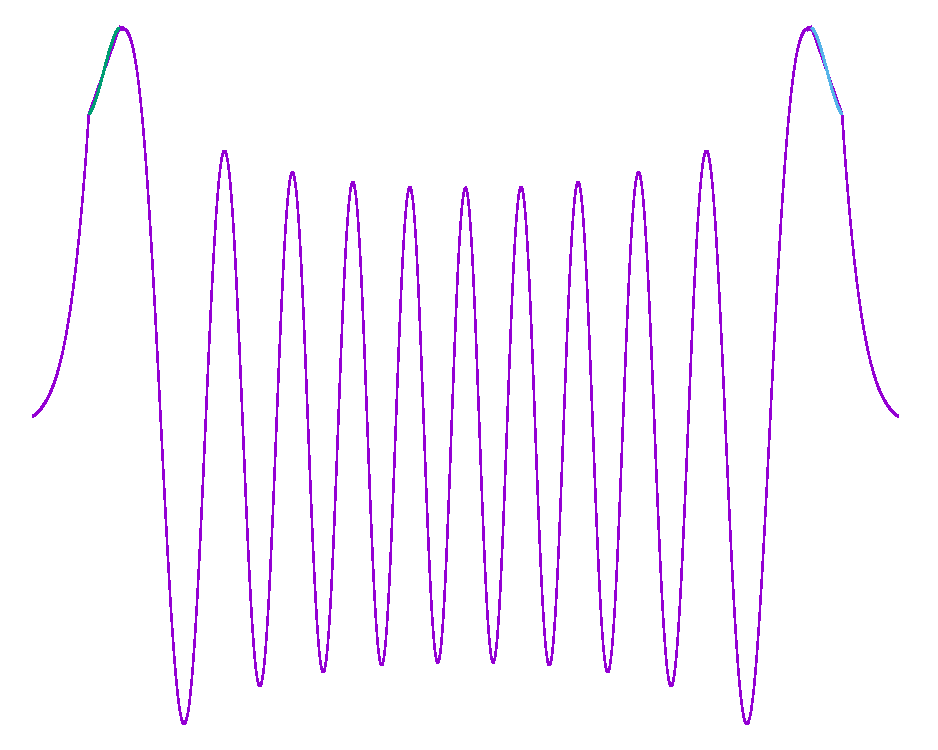
\includegraphics[width=.7\textwidth]{plots/wave_func_square.pdf}
\end{center}
\vspace{0.05\textheight}
Maturaarbeit\\
Kantonsschule Glarus\\
Betreuer: Linus Romer\\
Referent: Elena Borisova
\end{center}
\end{titlepage}

\pagenumbering{roman}   % i, ii, iii, iv, ...

\tableofcontents

\pagebreak[4]

\chapter*{Vorwort}
\addcontentsline{toc}{chapter}{\protect\numberline{}Vorwort}
Der Rest der Arbeit wird in Englisch sein aber ich habe mich entschieden eine kleine Zusammenfassung zu schreiben, so dass jeder zumindest die Grundlagen meiner Arbeit versteht.
Zu begin des 20. Jahrhunderts gab es einen Umschwung in der Physik, Quantenmechanik wurde entdeckt. Diese neue Theorie kann nicht mehr präzise voraussagen machen wie es zuvor der Fall war.
Man kann nur noch sagen mit welcher Wahrscheinlichkeit etwas passiert und ein Partikel kann an zwei Orten gleichzeitig sein.

Vielleicht haben Sie schon einmal von Schrödingers Katze gehört. Dies war ein Gedankenexperiment von Schrödinger um auf zu zeigen wie absurd seine Theorie wirklich ist und dass sie nicht stimmen könne.
Stell dir vor du schliesst deine Katze in eine Box ein. In dieser Box ist ein Atom das entweder zerfallen kann oder nicht. Dazu gibt es einen Detektor der misst ob das Atom zerfallen ist, in diesem Fall
wird ein Gift frei gelassen und die Katze stirbt.
Das Problem ist jetzt aber, dass dieses Atom den Regeln der Quanten Mechanik folgt und deshalb gleichzeitig bereits zerfallen ist und nicht zerfallen ist, die einzig logische Schlussfolgerung ist deshalb,
dass \emph{die Katze gleichzeitig Tod und am leben ist} \citep{schrodinger1935gegenwartige}.

In der Realität funktioniert es wahrscheinlich jedoch nicht so. Heisst das Universum ``entscheidet'' ob die Katze gestorben ist oder nicht, jedoch weiss man bis Heute nicht wann das Universum ``entscheidet''.

Damit die Katze gleichzeitig Tod und Lebendig sein kann brauchen wir die Wellenfunktion. Sie beschreibt alles was in unserem Universum gerade passiert und ``speichert'' wie wahrscheinlich es ist, dass die Katze tot ist.

In meiner Maturaarbeit habe ich ein Programm geschrieben das genau diese Wellenfunktion ausrechnet in einem sehr vereinfachten Universum. Weil ich schon lange mal wissen möchte wie genau dieses bizarre Objekt aussieht. Auf der Titel Seite ist eine dieser Wellenfunktionen abgebildet.

\pagebreak[4]

\chapter{Introduction}\pagenumbering{arabic}  % 1, 2, 3, 4, ...
Richard Feynmann one of the core people behind our modern theory of quantum mechanics repeatedly said: ``I think I can safely say that nobody understands quantum mechanics.''.
Nothing behaves like in our every day lives. Everything is just a probability and nothing certain.
Even Schrödinger the inventor of the equation that governs all of those weird phenomena rejected the idea that there are just probabilities.

In this paper we will try to understand this world a little bit better by looking at wave functions in a simplified universe.
This universe only has 1 dimension and there will not be any sense of time. This means we will be able to actually see how the wave function looks like in a graph.

\section{Goals}
The goal of this Maturaarbeit is to write a program, \bashinline{schroeding-approx} that calculates solutions to the time independent Schrödinger equation in 1 dimension for a large verity of potentials.
We assume that the wave function, $\Psi(x)$ will converge to 0 as $x$ goes to $\pm \infty$.
The program should be reasonably fast, meaning that for simple potentials and low energies
it should be done in under 1 minute.
The architecture should be able to support improvements.

Making the program user friendly is not a main focus. Meaning that a clear and simple API
that can be extended in the future is enough. Even dough the user will have to edit the code
to for example change between energies.

The program should also follow the UNIX philosophy, ``do one thing and one thing well''.
As a consequence the program will only do the calculations and not the plotting. But it
provides a simple and clear interface for a plotting program such as GNU Plot.

The main focus will be to balance performance and accuracy. Accuracy manly meaning that the
visualizations should be visually accurate and give some insight into quantum mechanics.
The user should also be able to tune the balance between performance and accuracy to some
degree.

\chapter{Preliminary}


\section{Schrödinger Equation}
In 1926 Erwin Schrödinger changed our understanding of quantum physics with the Schrödinger equation. Based on the observations of de Broglie that particles
behave like waves he developed a wave equation which describes how the waves move and change in a given potential $V(x)$ or Hamiltonian $\hat{H}$.
\begin{center}
\begin{math}
  \mi\hbar {\cfrac {\partial }{\partial t}}\Psi (x,t)=\left[-{\cfrac {\hbar ^{2}}{2m}}{\cfrac {\partial ^{2}}{\partial x^{2}}}+V(x,t)\right]\Psi (x,t)
\end{math}
\end{center}
Or more general
\begin{center}
\begin{math}
  \mi\hbar {\cfrac {\partial }{\partial t}}\Psi (x,t)=\hat{H} \Psi(x,t)
\end{math}
\end{center}

The time independent version that is going to be used later, ignores the change over time and is much simpler to solve since it is \emph{\textbf{only}} an ordinary differential equation instead of a
partial differential equation.
\begin{center}
\begin{math}
  E \psi (x)=\hat{H} \psi(x)
\end{math}
\end{center}
or
\begin{center}
\begin{math}
  -{\cfrac{\hbar^{2}}{2m}}  \cfrac{d^{2} \psi}{dx^{2}} (x) + V(x) \psi(x) = E \psi(x)
\end{math}
\end{center}

Even with the time independent equation it is very difficult to get analytical solutions, because of this there are mainly three approaches to
approximate solutions of $\psi(x)$, perturbation theory, density functional field theory and WKB approximation. Perturbation theory's goal is to give an analytical approximation which means it
is extremely difficult to implement for a computer. WKB on the other hand is much better since it is to some degree a step by step manual.
\section{Rust}
Rust is one of the newer programming languages and attempts to replace C/C++ which are notoriously difficult to work with. It supports both functional and object-oriented paradigms. It is much safer in terms of memory and promises the same performance as C. One of the goals of Rust is fearless concurrency which means everybody should
be able to write concurrent code without deadlocks and data races. This means calculations can utilize the full potential of the CPU without countless hours of debugging.

Functional programming languages are especially useful for mathematical problems, because they are based on the same mathematics as the problem.

Rust as of the time of writing this document is not yet standardized meaning the code provided might no longer be correct with one of the newer Rust versions.

In case you aren't familiar with Rust, it has excellent documentation on \url{https://doc.rust-lang.org/book/}.

\section{Interpretation of Quantum Mechanics}
The author believes in the many worlds interpretation of Hugh Everett. \emph{``The wave interpretation. This is the position proposed in the present thesis, in which the wave function itself is held to be
the fundamental entity, obeying at all times a deterministic wave equation.''} \citep[p. 115]{dewitt2015many}. This means that the observer is also quantum mechanical and gets entangled with one particular
state of the system that is being measured \citep[p. 116]{dewitt2015many}. This is some what different to the popular explanation of many worlds but has the same results and is, at least to the author
more reasonable.

An important point for the author also was that the theory accepts quantum mechanics as it is and doesn't make unreasonable assumption such as that the observer plays an important role.

On top of that this interpretation also discards the need for an ``observation'' in the program which would also be mathematically impossible \citep[p. 111]{dewitt2015many}.


\section{Complex Numbers}
In quantum mechanics it's customary to work with complex numbers. Complex numbers are an extension to the real numbers, since Rust will do most of the heavy lifting here are the most important things that you should know
\begin{align*}
  \mi^{2} = -1 \\
  z = a + b \mi \\
  \operatorname{Re}(z) = a \\
  \operatorname{Im}(z) = b \\
  \compconj{z} = a - b \mi \\
  \|z\|^{2} = a^{2} + b^{2} \\
  e^{\theta \mi} = \cos(\theta) + \mi \sin(\theta)
\end{align*}
$\mi$ is the imaginary unit,
$z$ is the general form of a complex number where $\{a,b\} \in \mathbb{R}$,
$\compconj{z}$ is the complex conjugate
and $\|z\|^{2}$ is the norm square of $z$.
The last equation is the Euler's formula, it rotates a number in the complex plane by $\theta$ radians.

The complex plane is similar to the real number line, every complex number can be represented on this plane where $\operatorname{Re}(z)$ is the x-coordinate and $\operatorname{Im}(z)$ is the y-coordinate.

\section{Gnuplot}
Gnuplot is a cross platform plotting program that is very simple to use. \bashinline{schroedinger-approx} will output a file \bashinline{data.txt}, you can plot the function by typing \bashinline{gnuplot}
and then typing
\begin{bashcode}
call "plot.gnuplot"
\end{bashcode}
to plot the real part of the wave function, or
\begin{bashcode}
call "plot_3d.gnuplot"
\end{bashcode}
to see the full complex wave function.

If you'd like to learn more about Gnuplot you can read there user manual on \url{http://www.gnuplot.info/}

\section{Planck Units}
By using Planck units the equations get a little bit easier.
Working in Planck units means that all fundamental constants are equal to 1.
\[
  c = k_{B} = G = \hbar = 1.
\]
This means that the constants will usually cancel out.

To convert to SI units we can just multiply powers of the constants such that there unit results in one of the base units.
\begin{align*}
l_{\text{Planck}} = l_{\text{SI}} \sqrt{\cfrac{G \hbar}{c^{3}}}  && 1~\text{m}_{\text{Planck}}  \approx 1.616255(18) \cdot 10^{-35}~\text{m}  && \text{\citep{CODATAValuePlanckLength}} \\
m_{\text{Planck}} = m_{\text{SI}} \sqrt{\cfrac{c \hbar}{G}}      && 1~\text{kg}_{\text{Planck}} \approx  2.176434(24) \cdot 10^{-8}~\text{kg} && \text{\citep{CODATAValuePlanckMass}} \\
t_{\text{Planck}} = t_{\text{SI}} \sqrt{\cfrac{G \hbar}{c^{5}}} && 1~\text{s}_{\text{Planck}}  \approx 5.391247(60) \cdot 10^{-44}~\text{s}  && \text{\citep{CODATAValuePlanckTime}}
\end{align*}
\hspace*{\fill}~\citep[Table 1]{gaarder2016gravitational} \\
\\
The program will take all of its in- and outputs in Planck units.

\chapter{Methods}
\section{Program Architecture}
The program has multiple interfaces or traits as they are called in Rust that give the program some abstraction.
In~\ref{fig:uml-arch} is a UML diagram of the architecture.
  \label{fig:uml-arch}
  \centering
  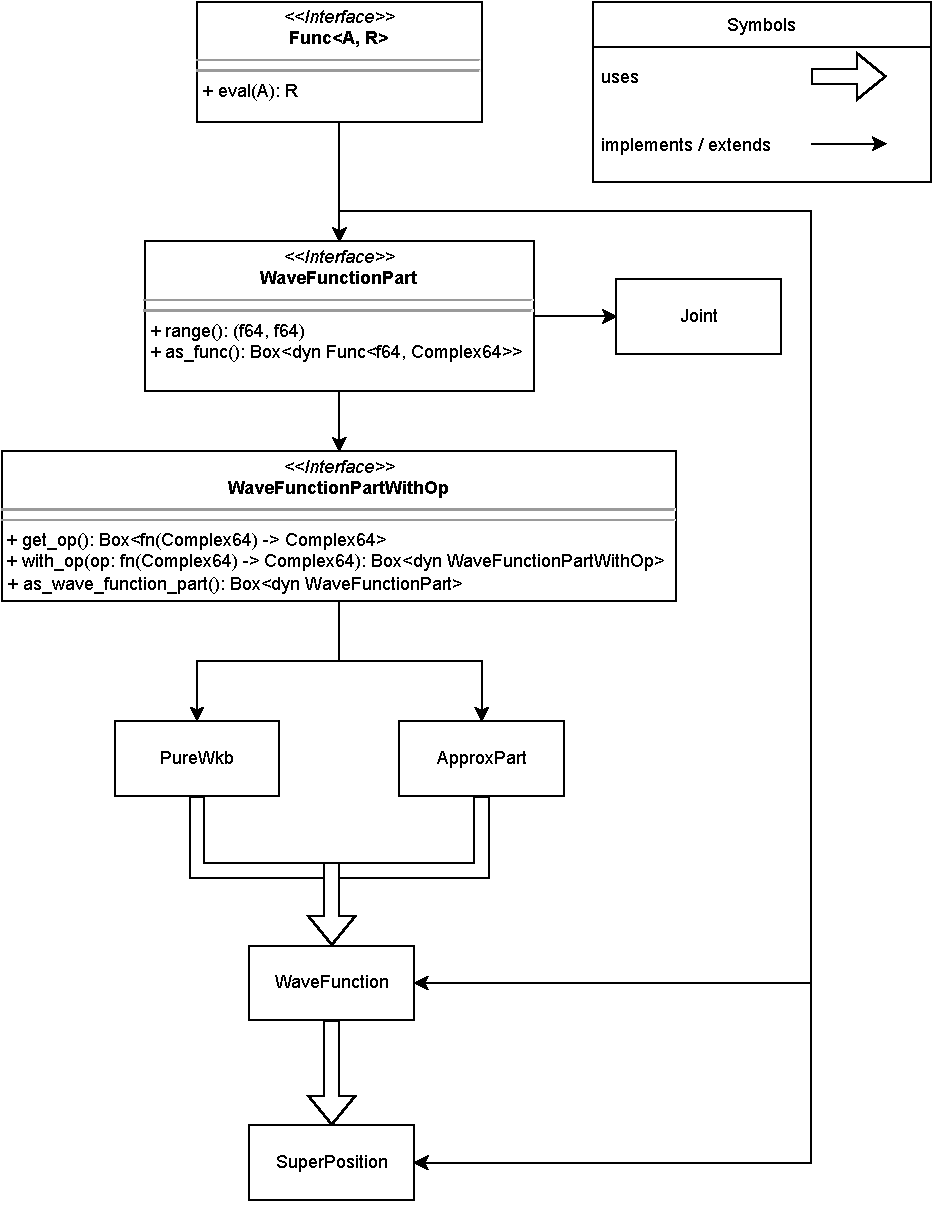
\includegraphics[width=\textwidth]{program_architecture.pdf}
  \caption{UML diagram of program architecture}
\end{figure}
Since current version of Rust does not support manual implementations of \rustinline{std::ops::Fn} we have to define our own trait for functions \rustinline{Func<A, R>} where \rustinline{A} is the type of the argument and \rustinline{R} is the return type. Later we will use this trait to implement functions for integration,evaluation and more useful utilities.

\rustinline{WaveFunction} is at the heart of the program, it contains all the functionality to build wave functions. It is composed of \rustinline{WaveFunctionPart} which represent either a \rustinline{Joint}, \rustinline{PureWkb} or an \rustinline{ApproxPart}. With the \rustinline{range} function we can check when they are valid.

\section{Newtons Method}
Newton's method, also called the Newton-Raphson method, is a root-finding algorithm that uses the first few terms of the Taylor series of a function $f(x)$ in the vicinity of a suspected root
\citep{math:newton}. It makes a sequence of approximations of a root $x_{n}$ that in certain cases converges to the exact value where
\[
  \lim _{n \to \infty}f(x_{n}) = 0
\]

The sequence is defined as
\begin{align*}
  x_{0}=a \\*
  x_{n+1}=x_{n}-\cfrac{f(x_{n})}{f'(x_{n})}
\end{align*}

Visually this looks like figure~\ref{fig:newton-ilust} $f(x) = (x-2)(x-1)(x+1)$.
\begin{figure}[H]
	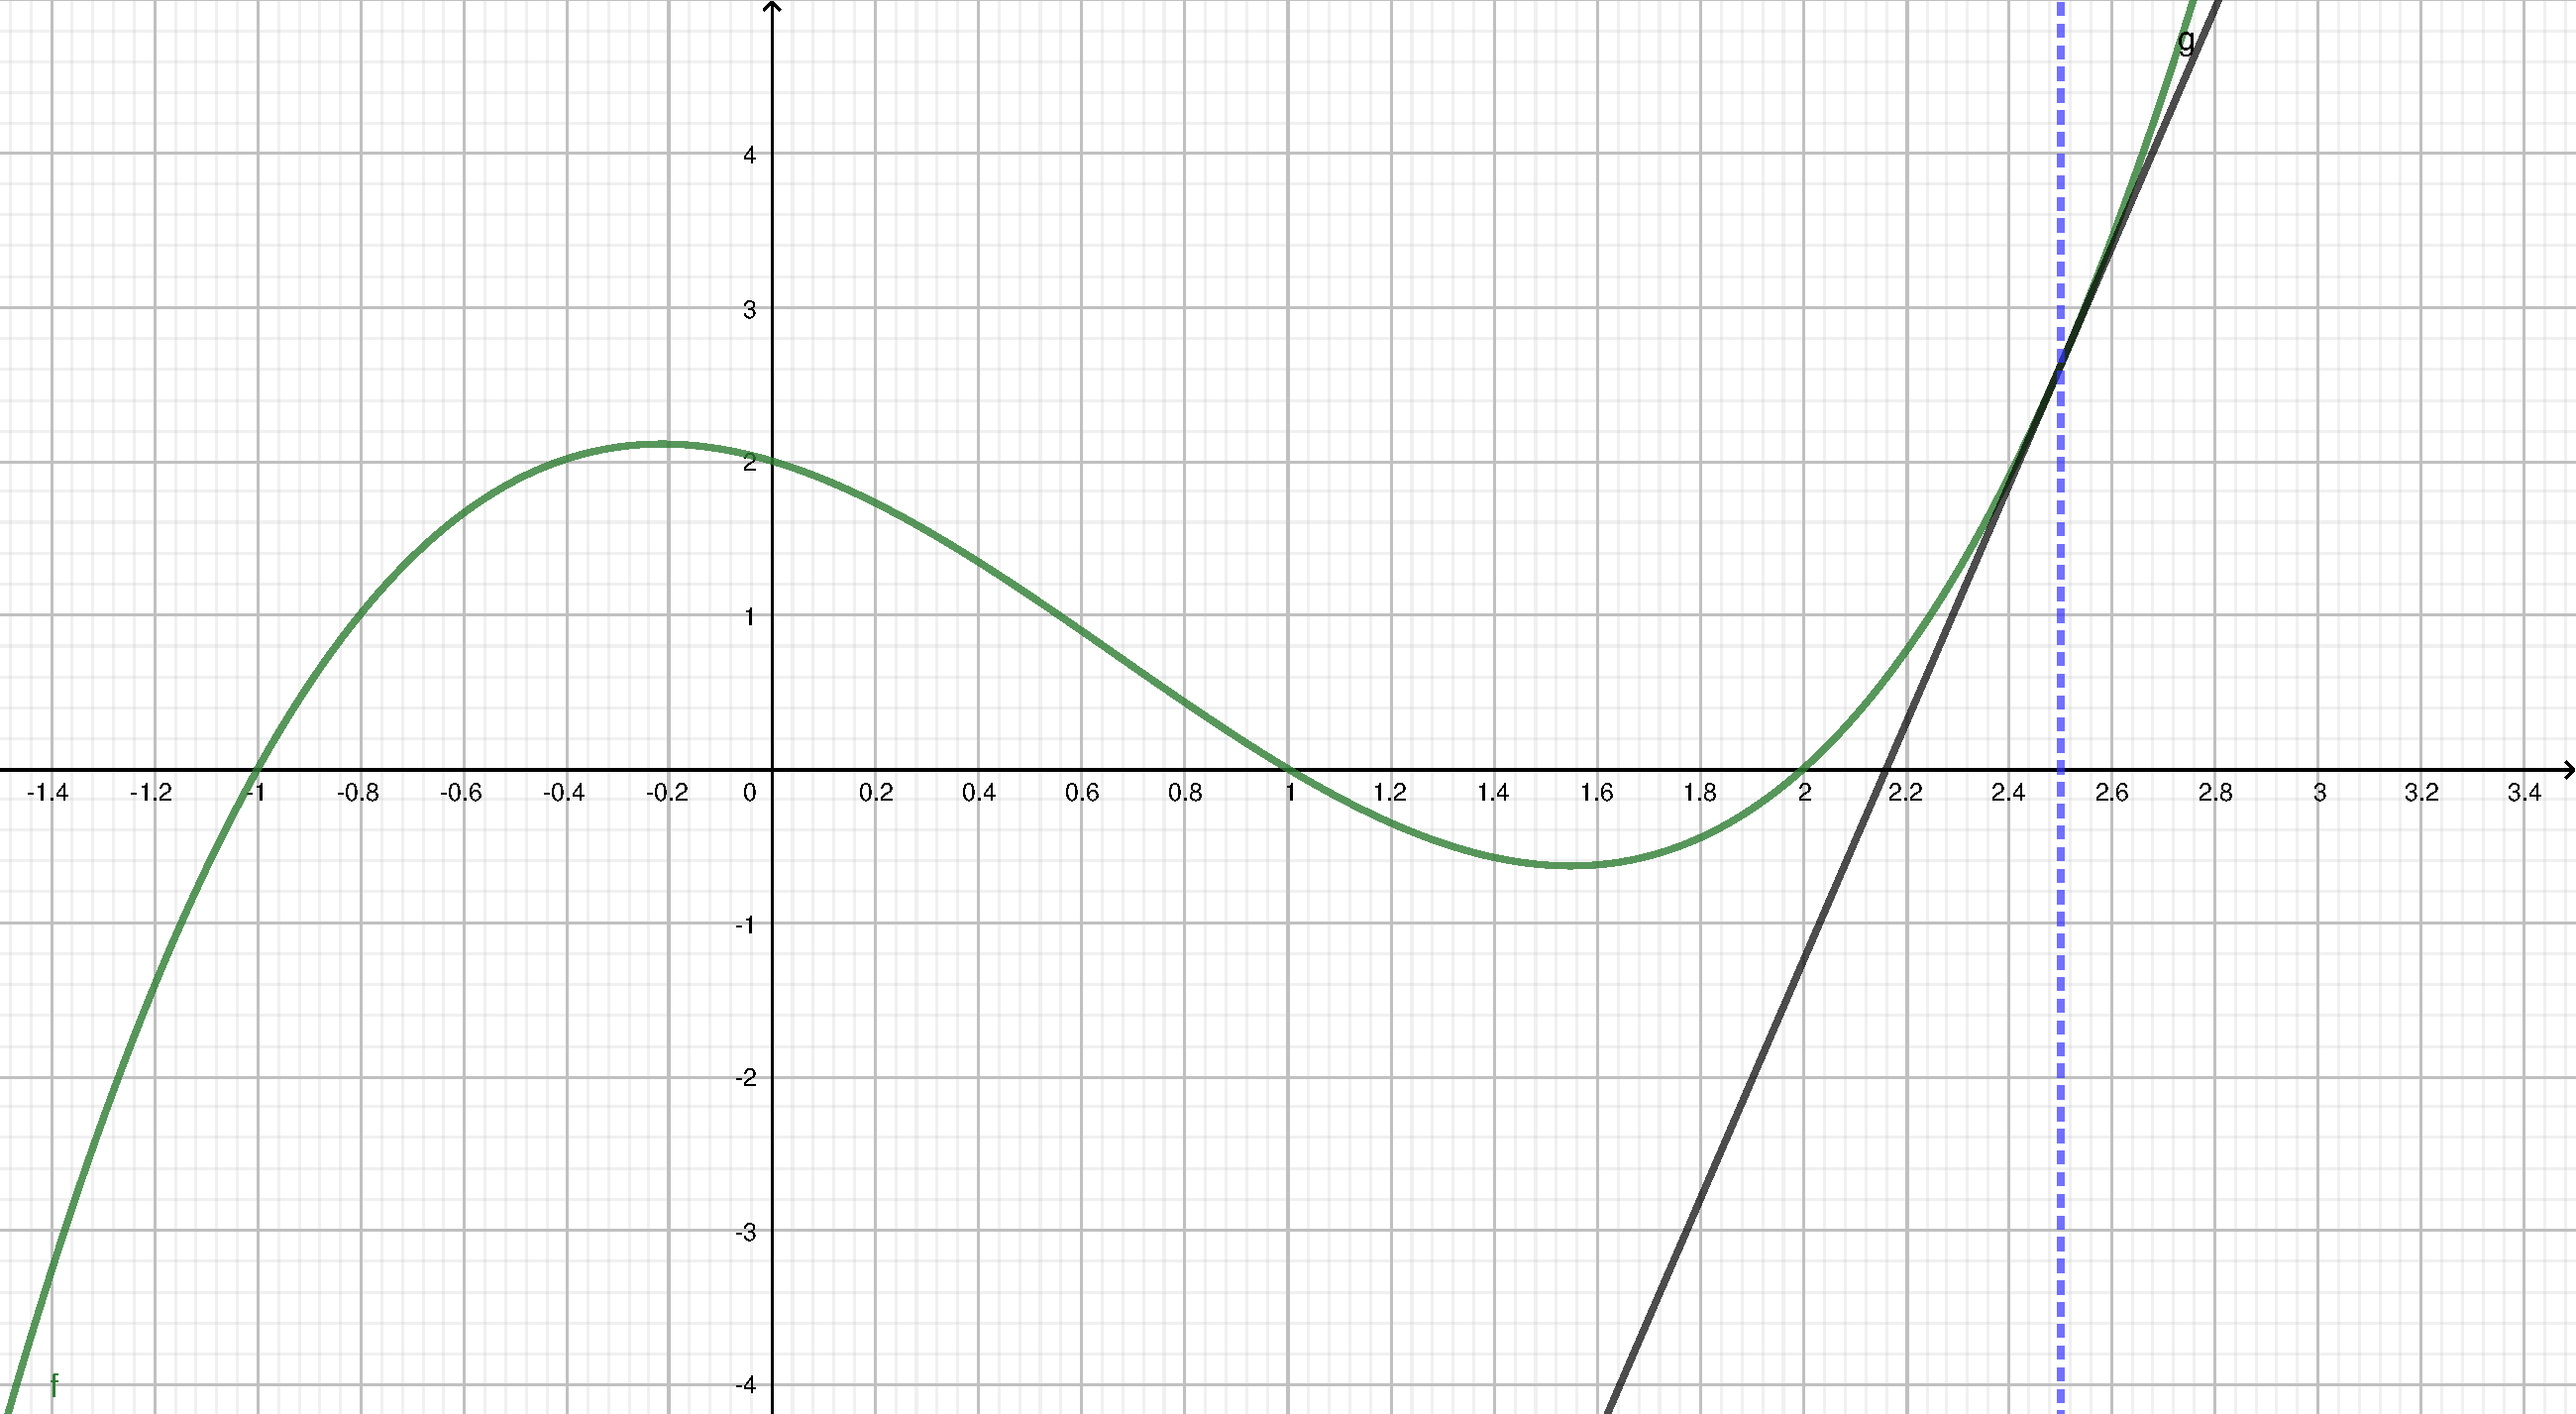
\includegraphics[width=\textwidth]{plots/newtons-method.pdf}
	\caption{Illustration of Newtons method, $f(x) = (x-1)(x-2)(x+1)$.}
	\label{fig:newton-ilust}
\end{figure}
The blue line indicates the initial guess which in this case is $2.5$ the black line ($g(x)$) is a tangent to $f(x)$ at $(guess, f(guess))$ the next guess will be where
the tangent intersects the x-Axis (solution of $g(x) = 0$). This will converge rather quickly compared to other methods such as Regula falsi.

\pagebreak
\begin{rustcode}\nopagebreak
pub fn newtons_method<F>(f: &F, mut guess: f64, precision: f64) -> f64
    where
        F: Fn(f64) -> f64,
{
    loop {
        let step = f(guess) / derivative(f, guess);
        if step.abs() < precision {
            return guess;
        } else {
            guess -= step;
        }
    }
}
\end{rustcode}

In Rust the sequence is implemented with a function that takes a closure \rustinline{f}, the initial guess \rustinline{guess} and a stop condition \rustinline{precision} the function will return if
$\|cfrac{f(x_{n})}{f'(x_{n})}|$ is less than \rustinline{precision}.

From the structure of the algorithm it is very tempting to implement it recursively, but by using a loop it is much faster since there are no unnecessary jumps and the precision can (at least in theory) be $0$ without causing a stack overflow.

\section{Regula Falsi with Bisection}
Newtons method fails if the first guess is at a maximum, since the step would go to infinity. For this case we can first use a bisection search to detect a sign change.
We need to do a bisection search since Regula falsi requires two guesses.

The algorithm itself is quite simple. To start we need
\begin{align}
  f(x): \mathbb{R} \to \mathbb{R} \\
  \{a \in \mathbb{R}~|~f(a) \le 0\} \\
  \{b \in \mathbb{R}~|~f(b) \ge 0\}.
\end{align}
Then we can draw a line between the two points $(a, f(a))$ and $(b, f(b))$. Then $a$ becomes
the x-value where the line intersects the x-axis becomes the new $b$, when we do the process
again with the new $b$ we will get our new value for $a$. We can repeat this process until we
cross a fresh hold for the accuracy and the result will be the last inter section of the line
with the x-axis.

\section{Derivatives}
Derivatives can be calculated numerically as in the C++ library Boost \citep{boost:calculating-derivative}.
The author implemented a analytical system for derivatives in Go. From that experience the
benefit is negligible compared to the increase in performance and in development time since
every function is a special object.

\begin{rustcode}
pub fn derivative<F, R>(func: &F, x: f64) -> R
where
    F: Fn(f64) -> R + ?Sized,
    R: Sub<R, Output = R> + Div<f64, Output = R> + Mul<f64, Output = R> + Add<R, Output = R>,
{
    let dx = f64::epsilon().sqrt();
    let dx1 = dx;
    let dx2 = dx1 * 2.0;
    let dx3 = dx1 * 3.0;

    let m1 = (func(x + dx1) - func(x - dx1)) / 2.0;
    let m2 = (func(x + dx2) - func(x - dx2)) / 4.0;
    let m3 = (func(x + dx3) - func(x - dx3)) / 6.0;

    let fifteen_m1 = m1 * 15.0;
    let six_m2 = m2 * 6.0;
    let ten_dx1 = dx1 * 10.0;

    return ((fifteen_m1 - six_m2) + m3) / ten_dx1;
}
\end{rustcode}
\rustinline{f64::epsilon().sqrt()} is approximately $0.000000014901161$.
\rustinline{f64::epsilon()} is the smallest double precision floating point number where $1 +
\epsilon \ne 1$. this has been chosen for $dx$ because it should be fairly precise.

\section{Integration}
The same principles apply to integrals as to derivative it would not be a great benefit to implement an analytic integration system. Integrals would also be much more difficult to implement than
derivatives since integrals can not be broken down in to many smaller integrals that can be computed easily instead it needs to be solved as is.

One approach would be to use the same method as with the derivative, take the definition with the limit and use a small value but this method can be improved in this case, since integrals calculate
areas under curves a trapeze is more efficient and accurate then the rectangle that results from the definition.

\begin{figure}[h]
  \centering
	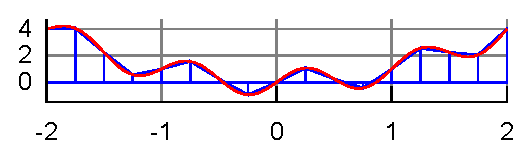
\includegraphics[width=0.7\textwidth]{plots/Integration_trapezoid.pdf}
	\caption{Illustration of integration with trapeze from \cite{wiki:integration-methods}.}
	\label{fig:integration-ilust}
\end{figure}

Figure~\ref{fig:integration-ilust} shows visually how the methods work, each blue trapeze from start ($a$) to end ($b$) has an area of
\[
\int _{a}^{b}f(x)\,dx\approx (b-a)f\left({\cfrac {a+b}{2}}\right).
\]
One trapeze would be fairly inaccurate to calculate the area under the function but as the area from $a$ to $b$ is subdivided further the result become better and better.

The general structure of the algorithm can very easily be run in parallel since it doesn't matter in which order the segments are added together and the segments also don't dependent on one another.
In Rust this is implemented using rayon. Rayon is an implementation for parallel iterators meaning that normal data structures that implement \rustinline{std::iter} can be run in parallel \emph{just} by
changing \rustinline{::iter()} to \rustinline{::par_iter()}. This might not work in all cases because of memory safety but in this case the borrow checker will throw an error and the code wont compile.

\begin{rustcode}
pub trait Func<A, R>: Sync + Send {
    fn eval(&self, x: A) -> R;
}

pub struct Point {
    pub x: f64,
    pub y: Complex64,
}
\end{rustcode}
Such that functions with states, like wave functions that store parameters, can be integrated
there is a trait \rustinline{Func<A, R>}.

\rustinline{Point} stores both the input, x and the output, y of a function.

\begin{rustcode}
pub fn evaluate_function_between<X, Y>(f: &dyn Func<X, Y>, a: X, b: X, n: usize) -> Vec<Point<X, Y>>
where
    X: Copy
        + Send
        + Sync
        + std::cmp::PartialEq
        + From<f64>
        + std::ops::Add<Output = X>
        + std::ops::Sub<Output = X>
        + std::ops::Mul<Output = X>
        + std::ops::Div<Output = X>,
    Y: Send + Sync,
{
    if a == b {
        return vec![];
    }

    (0..n)
        .into_par_iter()
        .map(|i| {
            index_to_range(
                X::from(i as f64),
                X::from(0.0_f64),
                X::from((n - 1) as f64),
                a,
                b,
            )
        })
        .map(|x: X| Point { x, y: f.eval(x) })
        .collect()
}
\end{rustcode}
\rustinline{Func<X, Y>} can be passed to \rustinline{evaluate_function_between}
it calculates \rustinline{n} points between an interval from \rustinline{a} to \rustinline{b}
and returns a vector of \rustinline{Point}. \rustinline{X} and \rustinline{Y} are general
data types such that it supports as many types of numbers as possible.

\pagebreak
\begin{rustcode}
pub fn integrate<
    X: Sync + std::ops::Add<Output = X> + std::ops::Sub<Output = X> + Copy,
    Y: Default
        + Sync
        + std::ops::AddAssign
        + std::ops::Div<f64, Output = Y>
        + std::ops::Mul<Output = Y>
        + std::ops::Add<Output = Y>
        + Send
        + std::iter::Sum<Y>
        + Copy
        + From<X>,
>(
    points: Vec<Point<X, Y>>,
    batch_size: usize,
) -> Y {
    if points.len() < 2 {
        return Y::default();
    }

    let batches: Vec<&[Point<X, Y>]> = points.chunks(batch_size).collect();

    let parallel: Y = batches
        .par_iter()
        .map(|batch| {
            let mut sum = Y::default();
            for i in 0..(batch.len() - 1) {
                sum += trapezoidal_approx(&batch[i], &batch[i + 1]);
            }
            return sum;
        })
        .sum();

    let mut rest = Y::default();

    for i in 0..batches.len() - 1 {
        rest += trapezoidal_approx(&batches[i][batches[i].len() - 1], &batches[i + 1][0]);
    }

    return parallel + rest;
}
\end{rustcode}
The actual integration happens in \rustinline{integrate}, it calculates the areas of the trapezes between the points passed to it. For optimization 1000 trapezes are calculated per thread because it would
take more time to create a new thread then to actually do the calculation, this has to be further investigated and 1000 might not be optimal. The calculations performed per thread are called a batch,
after all batches have been calculated the boundaries between batches also has to be considered therefor they are added in the end with \rustinline{rest}.

\section{Transition Regions}
The approximation that will be used splits $\Psi(x)$ into multiple parts that do not match perfectly together.

\begin{figure}[h]\label{fig:cos_taylor}
  \centering
  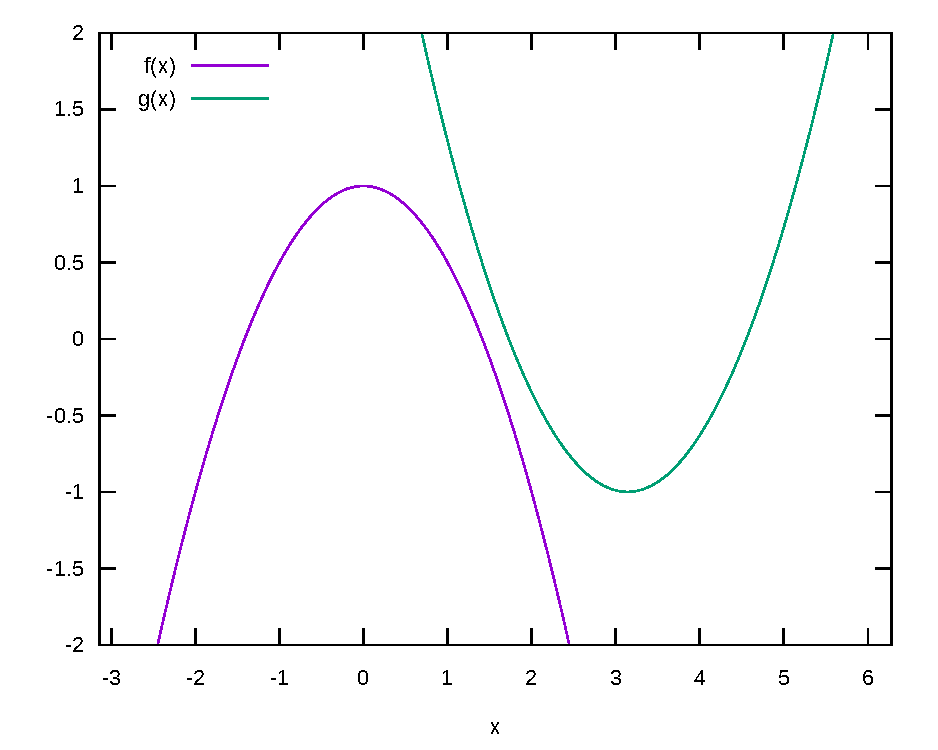
\includegraphics[width=.9\textwidth]{plots/cos_taylor.pdf}
  \caption{Example for joining functions}
\end{figure}

Lets consider an example, in figure \ref{fig:cos_taylor} we can see two Taylor series of cosine. Now we have to join the two functions at $x = \pi / 2$ such that its a mathematically smooth transition.
\begin{align}
  \label{joint:f}
  f(x) = 1 - \cfrac{x^{2}}{2} \\
  \label{joint:g}
  g(x) = \cfrac{(x - \pi)^{2}}{2} -  1
\end{align}

As a first guess lets join $f(x)$ and $g(x)$ with a step function, this means that the joint function $h(x)$ will be
\[
  h(x) =  \left\{
    \begin{array}{ll}
           f(x) & x < \cfrac{\pi}{2} \\
           g(x) & x > \cfrac{\pi}{2}
    \end{array}
    \right..
\]
This gives us~\ref{fig:joint-step} which is obviously not smooth.
\begin{figure}[H]\label{fig:joint-step}
  \centering
  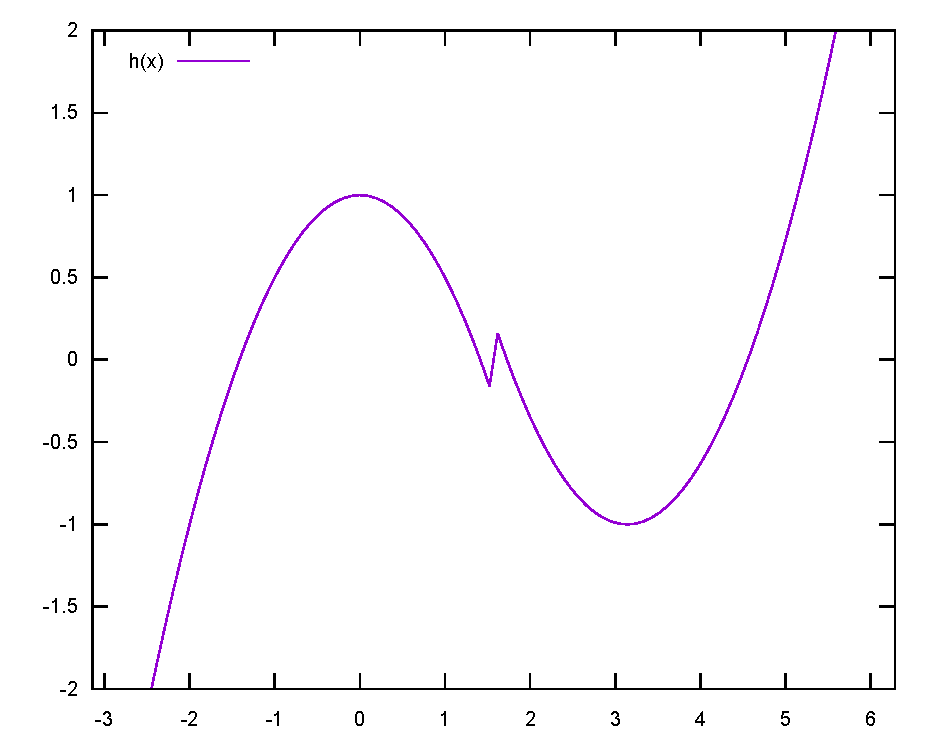
\includegraphics[width=.9\textwidth]{plots/step_joint.pdf}
  \caption{Plot of h(x) with step joint}
\end{figure}

If we use the formula from~\cite[p. 325, section 15.6.4]{hall2013quantum} with
\begin{align*}
    \delta = 0.5 \\
    \alpha = \cfrac{\pi}{2} - \cfrac{\delta}{2} \\
    \chi(x) = \sin^{2}\left(x \cfrac{\pi}{2}\right)
\end{align*}
this results in
\[
  h(x) =  \left\{
    \begin{array}{ll}
      f(x) & x < \alpha \\
      g(x) & x > \alpha + \delta \\
      f(x) + (g(x) - f(x))\chi(\cfrac{x-\alpha}{\delta}) & else
    \end{array}
    \right.
\]
which is mathematically smooth as we can see in figure~\ref{fig:joint-cos-hall} (proof in Appendix~\ref{proof:joint}).
\begin{figure}[H]\label{fig:joint-cos-hall}
  \centering
  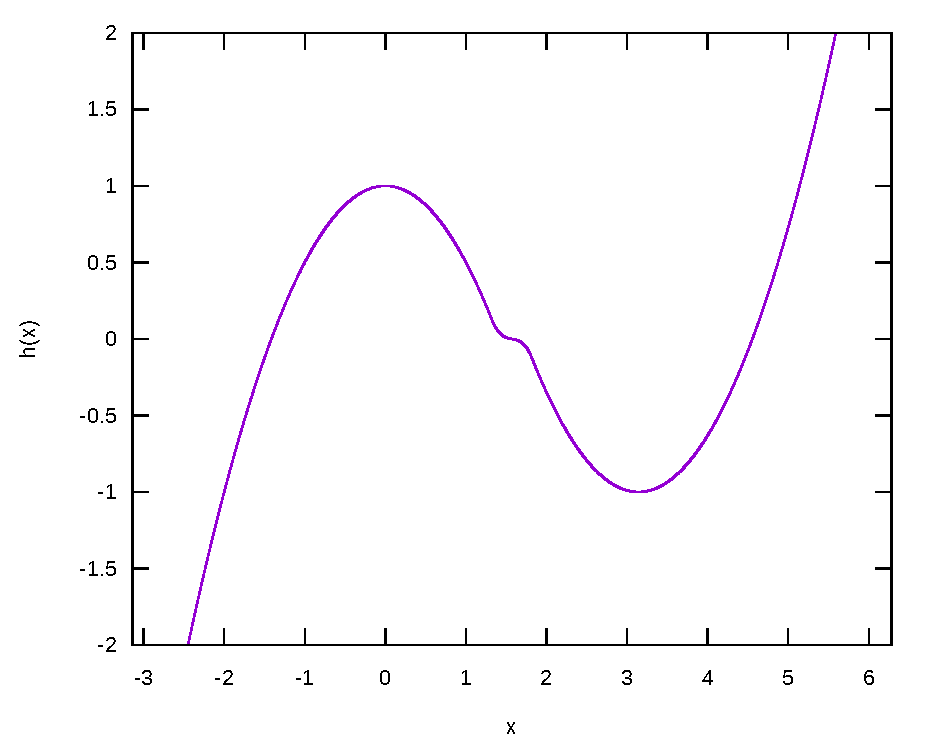
\includegraphics[width=.9\textwidth]{plots/hall_joint.pdf}
  \caption{Plot of h(x) with Hall joint}
\end{figure}

\subsection{Implementation in Rust}
In the program we can define a struct \rustinline{Joint} that implements \rustinline{Func<f64, Complex64>}. As in the example we need two functions $f(x)$ and $g(x)$ which we will rename to \rustinline{left} and \rustinline{right}. We will also need a variable $\alpha$ and $\delta$ which will be named \rustinline{cut} and \rustinline{delta}.
\begin{rustcode}
#[derive(Clone)]
pub struct Joint {
    pub left: Arc<dyn Func<f64, Complex64>>,
    pub right: Arc<dyn Func<f64, Complex64>>,
    pub cut: f64,
    pub delta: f64,
}

impl Func<f64, Complex64> for Joint {
    fn eval(&self, x: f64) -> Complex64 {
        let chi = |x: f64| f64::sin(x * f64::consts::PI / 2.0).powi(2);
        let left_val = left.eval(x);
        return left_val + (right.eval(x) - left_val) * chi((x - self.cut) / self.delta)
    }
}
\end{rustcode}

In the proof we assume that $f(x)$ and $g(x)$ are continuous of first order in the interval $(\alpha, \alpha + \delta)$. In the code we will not check this requirement since it would have a major impact on performance to check the derivative on every point.

\chapter{Calculation}
\section{Energy Levels}
Solving the Schrödinger equation is an eigenvalue problem. This means that only certain energies will result in physically correct results. For an energy to be valid it has to satisfy the Maslov-corrected Bhor-Sommerfeld condition which states that
\begin{align}
  n \in \mathbb{N}_{0}\\
  C = \left\{x \in \mathbb{R}~|~V(x) < E \right\}\\
  \int_{C}\sqrt{2m(E - V(x))}dx = 2\pi(n + 1/2)
\end{align}\emph{this condition does not (in most cases) give the exact energy levels}~\citep{hall2013quantum}.
It can be interpreted such that the oscillating part of the wave function has to complete all half oscillation.

To solve this problem for an arbitrary potential in a computer the set $C$ and the fact that $n$ has to be a non negative integer is not really helpful, but the condition can be rewritten to
\begin{align}
  p(x) = \left\{\begin{array}{ll}
                  \sqrt{2m(E - V(x))} & V(x) < E \\
                  0 & else
                \end{array}
                      \right. \\\label{eq:prog_cond}
  \cfrac{1}{2\pi}\int_{-\infty}^{\infty}p(x) dx - \cfrac{1}{2} \mod{1} = 0
\end{align}
Unfortunately~\ref{eq:prog_cond} is not continuous which means that Newtons method can't be applied. Further on the bounds of integration have to be finite, this means the user of the program will have to
specify a value for the constant \rustinline{APPROX_INF} where any value for $x$ out side of that range should satisfy $V(x) > E$. But it shouldn't be to big since the \rustinline{integrate} function can only evaluate a relatively small number (default 64000) of trapezes before the performance will suffer enormously. The default value for \rustinline{APPROX_INF} is \rustinline{(-200.0, 200.0)}.

The implementation is quite strait forward we evaluate \ref{eq:prog_cond} for a number of energies and then check for discontinuities.
\begin{rustcode}
pub fn nth_energy<F: Fn(f64) -> f64 + Sync>(n: usize, mass: f64, pot: &F, view: (f64, f64)) -> f64 {
    const ENERGY_STEP: f64 = 10.0;
    const CHECKS_PER_ENERGY_STEP: usize = INTEG_STEPS;
    let sommerfeld_cond = SommerfeldCond { mass, pot, view };

    let mut energy = 0.0;
    let mut i = 0;

    loop {
        let vals = evaluate_function_between(
            &sommerfeld_cond,
            energy,
            energy + ENERGY_STEP,
            CHECKS_PER_ENERGY_STEP,
        );
        let mut int_solutions = vals
            .iter()
            .zip(vals.iter().skip(1))
            .collect::<Vec<(&Point<f64, f64>, &Point<f64, f64>)>>()
            .par_iter()
            .filter(|(p1, p2)| (p1.y - p2.y).abs() > 0.5 || p1.y.signum() != p2.y.signum())
            .map(|ps| ps.1)
            .collect::<Vec<&Point<f64, f64>>>();
        int_solutions.sort_by(|p1, p2| cmp_f64(&p1.x, &p2.x));
        if i + int_solutions.len() > n {
            return int_solutions[n - i].x;
        }
        energy += ENERGY_STEP - (ENERGY_STEP / (CHECKS_PER_ENERGY_STEP as f64 + 1.0));
        i += int_solutions.len();
    }
}
\end{rustcode}
First we check over the interval \rustinline{(0.0, ENERGY_STEP)} if there are not enough zeros we check the next interval of energies and so on until we found $n$ zeros.
It's also possible that \ref{eq:prog_cond} is negative before the 0th energy there for we also have to check for normal zeros by comparing the signs of the values.

The struct \rustinline{SommerfeldCond} is a \rustinline{Func<f64, f64>} that evaluates~\ref{eq:prog_cond}.

\subsection{Accuracy}
For a benchmark we will use
\begin{align*}
  m = 1 \\
  V(x) = x^{2} \\
  (-\infty, \infty) \approx (-200, 200).
\end{align*}
To get the actual values we will use Wolfram Language with WolframScript a programing language similar to Wolframalpha that can calculate the integral analytically.
In Rust we can rewrite \rustinline{main} to
\begin{rustcode}
fn main() {
    let output_dir = Path::new("output");

    let values = (0..=50)
        .into_iter()
        .map(|n: usize| Point::<usize, f64> {
            x: n,
            y: energy::nth_energy(n, 1.0, &potentials::square, APPROX_INF),
        })
        .collect::<Vec<Point<usize, f64>>>();

    std::env::set_current_dir(&output_dir).unwrap();
    File::create("energy.txt")
        .unwrap()
        .write_all(plot::to_gnuplot_string(values).as_bytes())
        .unwrap();
}
\end{rustcode}
This will output all energy levels from $n = 0$ to $n = 50$.
We can implement the same thing WolframScript

\begin{wslcode}
m = 1
V[x_] = x^2

nthEnergy[n_] = Module[{energys, energy},
    sommerfeldIntegral[en_] = Integrate[Sqrt[2*m*(en - V[x])],
                                            {x, -Sqrt[en], Sqrt[en]}]
    energys =  Solve[sommerfeldIntegral[en] == 2*Pi*(n + 1/2), en] // N;
    energy = en /. energys[[1]];
    energy
    ]

energys = Table[{n, N@nthEnergy[n]}, {n, 0, 50}]

csv = ExportString[energys, "CSV"]
csv = StringReplace[csv, "," -> " "]
Export["output/energies_exact.dat", csv]
\end{wslcode}
These programs will output two files \bashinline{energy.txt}~(Appendix~\ref{dat:energy-rs}) for our implementation in Rust and \bashinline{energies_exact.dat}~(Appendix~\ref{dat:energy-wsl}) for
WolframScript. As a ruff estimate we would expect an error of $\pm \cfrac{10}{64000} \approx \pm 1.56 * 10^{-4}$, because the program checks for energies with that step size.

\begin{figure}[H]\label{fig:energy-error}
  \centering
  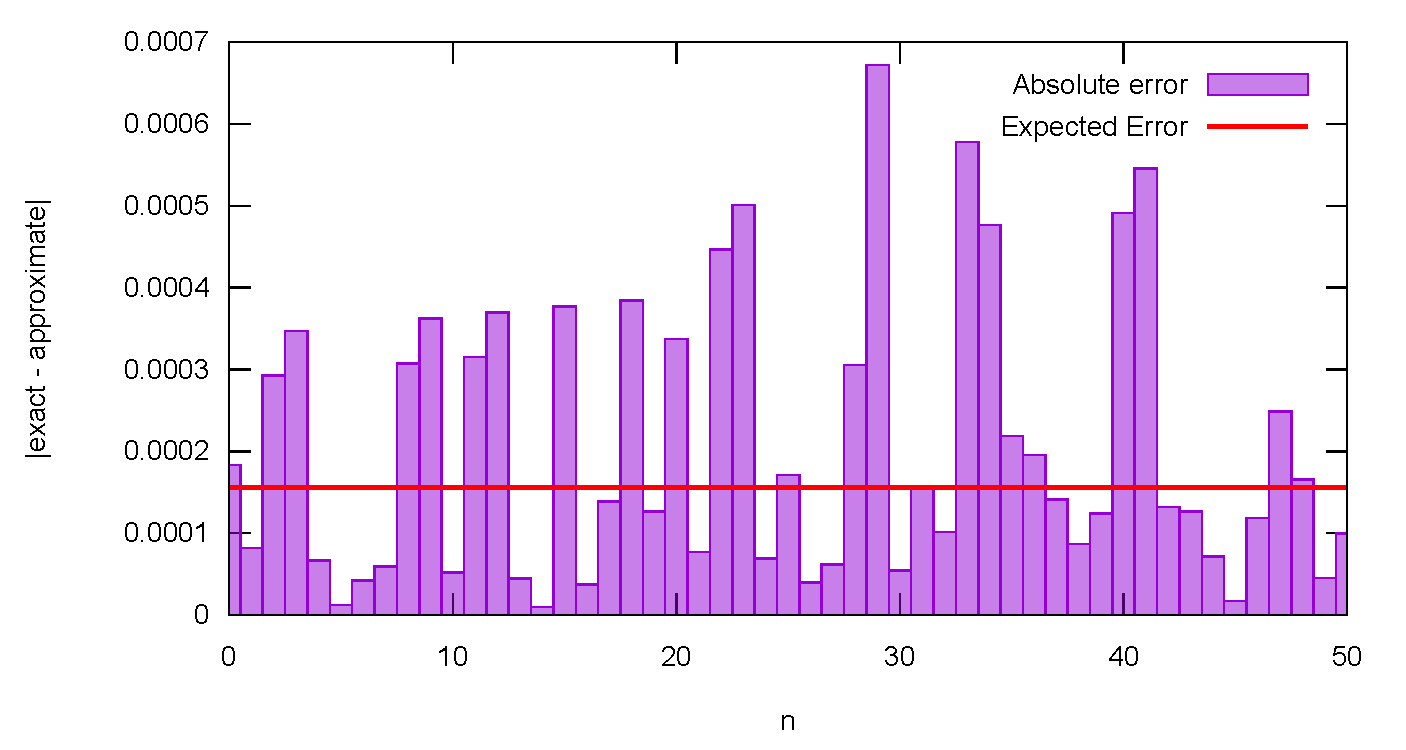
\includegraphics[width=\textwidth]{plots/energy_error.pdf}
  \caption{Absolute error of energy levels in square potential}
\end{figure}
When we plot the absolute error we get figure~\ref{fig:energy-error}. The error is a little higher than expected which is probably due to errors in the integral. Still the algorithm should be precise
enough. If you'd like you could pick a lower value for \rustinline{ENERGY_STEP} in \bashinline{src/energy.rs:49}, but this will impact the performance for calculating energies with higher numbers for $n$.


\section{Approximation Scheme}\label{meth:wkb:approximation-scheme}
There are mainly three approximation methods used to solve for the actual wave function itself. There is perturbation theory which breaks the problem down in to ever smaller sub-problems that then can be
solved exactly. This can be achieved by adding something to the Hamiltonian operator $\hat{H}$ which can then be solved exactly. But \textit{perturbation theory is inefficient compared to other approximation
methods when calculated on a computer} \citep[Introduction]{van2014density}.

The second is Density functional field theory, it has evolved over the years and is used heavily in chemistry to calculate properties of molecules and is also applicable for the time dependent Schrödinger
equation. It is something that might be interesting to add to the program in the future.
\\

The program uses the third method WKB approximation, it is applicable to a wide verity of linear differential equations and works very well in the case of the Schrödinger equation.
Originally it was developed by Wentzel, Kramers and Brillouin in 1926. It gives an approximation to the eigenfunctions of the Hamiltonian $\hat{H}$ in one dimension. The approximation is best
understood as applying to a fixed range of energies as $\hbar$ tends to zero \citep[p.~305]{hall2013quantum}.
\\

WKB splits $\Psi(x)$ into tree parts that can be connected to form the full solution. The tree parts are described as
\begin{align}
\label{eq:wkb:momentum}
  p(x) = \sqrt{2m(|E - V(x)|)} \\
\label{eq:wkb:t}
  V(t) - E = 0 \\
\label{eq:wkb:exp}
  \psi^{WKB}_{exp}(x)= \cfrac{c_{1}}{2 \sqrt{p(x)}} \exp\left(-\left|\int_{x}^{t}p(y) dy\right|\right) \\
\label{eq:wkb:osz}
  \psi^{WKB}_{osz} (x)= \cfrac{c_{1}}{\sqrt{p(x)}} \cos\left(\int_{x}^{t}p(y) dy - \delta \right) \\
  u_{1} = -2 m \cfrac{dV}{dx}(t) \\
\label{eq:airy}
  \psi^{Airy}(x) = \cfrac{c_{1} \sqrt{\pi}}{\sqrt[6]{u_{1}}} \operatorname{Ai}\left(\sqrt[3]{u_{1}} (t - x)\right).
\end{align}

Since equation \ref{eq:wkb:t} might have more than one solution for turning points $t$, we have to consider each one of them individually and in the end join them into one function.

The factor of $1/2$ in equation~\ref{eq:wkb:exp} is analogous to \citep[eq. 92]{robert2020wkb}. This means that it's only valid if the turning points aren't ``too close together''~\citep{robert2020wkb}.
This will be a problem later when we look at some solutions. \cite{robert2020wkb} also mansions that there are extensions to WKB that can handle these cases. It would be interesting to add those to the
program in the future.

\begin{figure}[H]\label{fig:wave_parts}
  \centering
  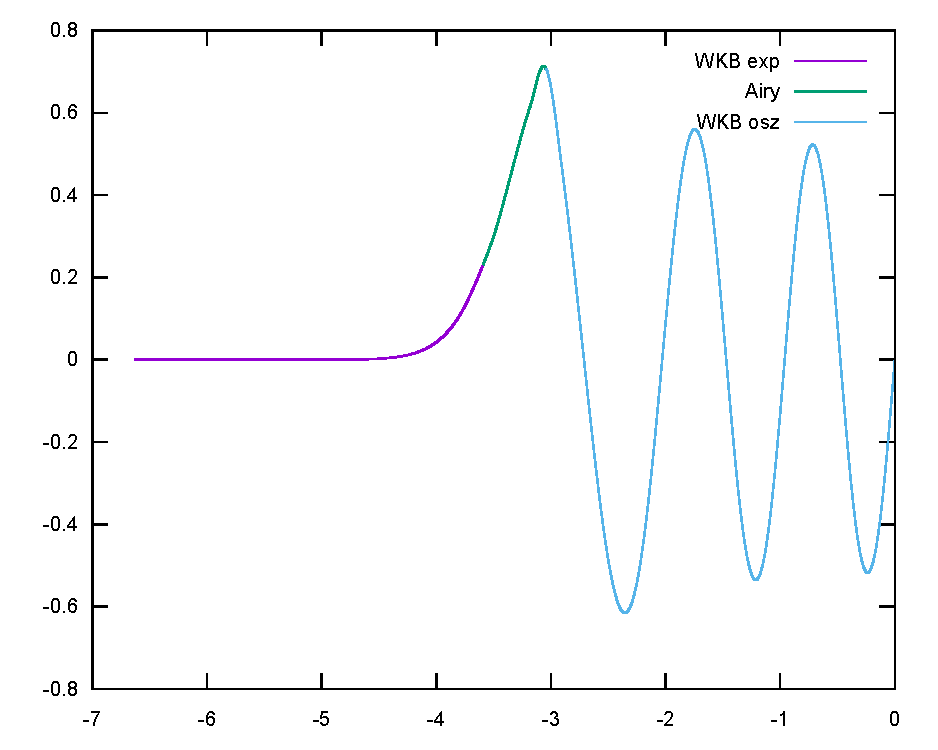
\includegraphics[width=.9\textwidth]{plots/square5half.pdf}
  \caption{Left half of wave function with $N_{Energy} = 5 \Rightarrow E = 11.0$, $m = 2$, $V(x) = x^{2}$}
\end{figure}
In figure~\ref{fig:wave_parts} the three parts are visualized. The purple section on the left is the exponential decaying part $\psi^{WKB}_{exp} (x)$, equation \ref{eq:wkb:exp} is a modified version of the
original version as described in \cite[p. 317, eq. 15.25]{hall2013quantum} where $b$ and $a$ are different solutions for $t$ of equation~\ref{eq:wkb:t}. The absolute symbol makes it possible to not
differentiate between the case where $x < t$ and $x > t$. Further on a factor of $e^{\delta\mi}$ was added such that the imaginary part of $\psi^{WKB}_{exp}(x)$ is the same as in $\psi^{WKB}_{osz}(x)$.

The blue part on the right is $\psi^{WKB}_{osz}(x)$. Again equation \ref{eq:wkb:osz} was expanded to result in the more general complex solution and it also works for both $\psi_{1}$ and $\psi_{2}$ in
\cite[p. 316-317, Claim 15.7]{hall2013quantum}. \cite{hall2013quantum} assumes that $\delta = \pi / 4$ which doesn't work in the simple case of $V(x) = x^{2}$, in figure \ref{fig:wave_parts} $\delta = 0$ was used. This will be further discussed in section \ref{...}.

\subsection{Validity}
When we look at the derivation of WKB we will see that equations \ref{eq:wkb:exp} and \ref{eq:wkb:osz} can only be valid if
\begin{align*}
  p(x) = \sqrt{V(x) - E} \\
  \left|\frac{dp}{dx}(x)\right| \ll p^{2}(x)
\end{align*}
as~\cite{zwiebach2018lecture} showed in his lecture.
But this would mean that WKB is only valid iff $V(x) > E$ because $p^{2}(x)$ would be negative otherwise.
If this is the case this would imply that~\ref{eq:wkb:exp} can't be valid.

We will assume that this contradiction is wrong and assume that WKB is valid if
\[
  \left|\frac{d}{dx}(\sqrt{|V(x) - E|})\right| < |V(x) - E|
\]

\subsection{Implementation}

\section{Turning Points}
A point $x$ where $V(x) = E$ is called a turning point. We assume that the WKB function is a good approximation in the region where
\begin{align}
  \label{eq:valid}
  -\cfrac{1}{2m} \deriv{V}{x}(x) \ll (V(x) - E)^{2}.
\end{align}
In order to do the actual calculation we need a range were the Airy function is valid.
From equation~\ref{eq:valid} we can infer that the Airy function is valid where
\begin{align}
  \label{eq:valid-airy}
  -\cfrac{a}{2m} \deriv{V}{x}(x) - (V(x) - E)^{2} > 0
\end{align}
We can assume that the Airy function is only valid in a closed interval, this means that there must be at least two roots of equation~\ref{eq:valid-airy}. These roots will be called turning point boundaries from now on. The factor of $a$ is used to emulate the behavior of $\ll$.

The left boundary point must have a positive and the right a negative derivative. This means we can solve for roots and group them together by there derivatives.
\\
In order to find all roots we will use a modification of Newtons method. When we find a solution, $x_{0}$ we can divide the original function by $(x - x_{0})$ this means that Newtons method wont be able to find $x_{0}$ again.

Further on since we check for roots inside the interval of \rustinline{APPROX_INF} we don't
have a good first guess where the turning point might be. Because of this we will make $1000$
guesses evenly distributed over the interval and invent a system that can rate how good of a
guess this point could be.
Newtons method works well if the value of $f(x)$ is small and $f'(x)$ is neither to small nor to big. We will assume that $f'(x) = 1$ is optimal.
As a rating we will use
\[
  \label{eq:rating-newton}
  \sigma(x) = \cfrac{|f(x)| }{ -\exp\left({{\left(\deriv{f}{x}(x)\right)}^{2} + 1}\right)}
\]
where lower is better. This function is just an educated guess, but it has to have some properties, as the derivative of $f$ tends to 0, $\sigma(x)$ should diverge to infinity.
\[lim_{\deriv{f}{x} \to 0} \sigma(x) = \infty\]
If $f(x) = 0$ we found an actual root in the first guess meaning that $\sigma(x)$ should be 0.
Formula~\ref{eq:rating-newton} doesn't satisfy this property since it's undefined if $f'(x) = 0$ and $f(x) = 0$, but we can extend it's definition such that
\[
  \sigma(x) = \left\{
    \begin{array}{ll}
    \cfrac{|f(x)| }{ -\exp\left({{\left(\deriv{f}{x}(x)\right)}^{2} + 1}\right)} & f(x) \ne 0~\text{and}~\deriv{f}{x} \ne 0 \\
    0 & \text{else}
    \end{array}\right.
\]

\begin{figure}[H]\label{fig:simga-heat}
  \centering
  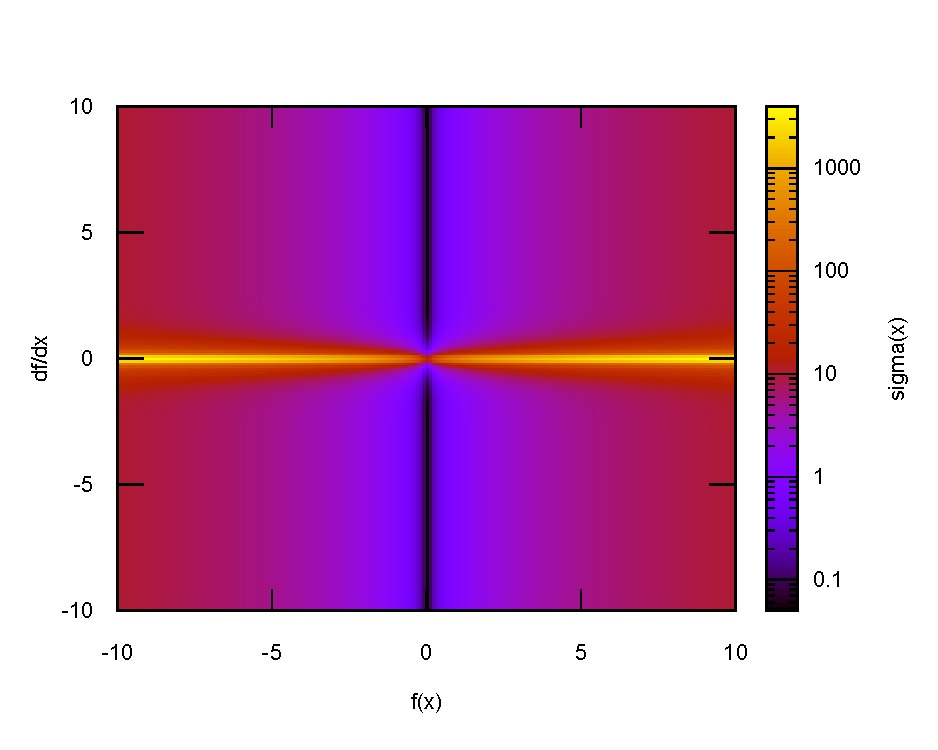
\includegraphics[width=0.9\textwidth]{plots/newton_rating_func.pdf}
  \caption{Logarithmic heat diagram of $\sigma(x)$, darker/bluer is better}
\end{figure}
As we can see in figure~\ref{fig:simga-heat} where darker/bluer values are better than yellow/red areas that $\sigma(x)$ indeed has all of the desired properties.
\\
\\
After we rated all of the 1000 guesses we can pick the best one as a first guess and use the modified Newtons method with it. We do this process 256 times by default. In theory we could therefor use the WKB approximation for potentials with up to 256 turning points.

\begin{rustcode}
fn find_zeros(phase: &Phase, view: (f64, f64)) -> Vec<f64> {
    let phase_clone = phase.clone();
    let validity_func = Arc::new(move |x: f64| {
        1.0 / (2.0 * phase_clone.mass).sqrt() * derivative(&|t| (phase_clone.potential)(t), x).abs()
            - ((phase_clone.potential)(x) - phase_clone.energy).pow(2)
    });
    let mut zeros = NewtonsMethodFindNewZero::new(validity_func, ACCURACY, 1e4 as usize);

    (0..MAX_TURNING_POINTS).into_iter().for_each(|_| {
        let modified_func = |x| zeros.modified_func(x);

        let guess = make_guess(&modified_func, view, 1000);
        guess.map(|g| zeros.next_zero(g));
    });

    let view = if view.0 < view.1 {
        view
    } else {
        (view.1, view.0)
    };
    let unique_zeros = zeros
        .get_previous_zeros()
        .iter()
        .filter(|x| **x > view.0 && **x < view.1)
        .map(|x| *x)
        .collect::<Vec<f64>>();
    return unique_zeros;
}
\end{rustcode}
Here \rustinline{make_guess} uses $\sigma(x)$ and returns the best guess. \rustinline{NewtonsMethodFindNewZero} is the modified version of Newtons method where all the roots are stored and its
implementation of \rustinline{Func<f64, f64>} is just defined as
\begin{align}
  \label{eq:newton-modified}
  \cfrac{f(x)}{\prod\limits_{r \in Z} (x - r)}
\end{align}
Where the set $Z$ is the set of all the zeros that have been found previously.
After the 256 iterations we filter out all the zeros that aren't in the view.
Equation~\ref{eq:newton-modified} is implemented in \rustinline{NewtonsMethodFindNewZero}.
Unfortunately this procedure can't be implement asynchronously since you have to know all
previous zeros before you can find a new one.

Once we found the zeros we need to group them as previously mentioned the derivative of the
validity function (\ref{eq:valid-airy}) must be positive if the boundary point is on the left
and negative when its on the right side of the turning point.
It could be the case that if the turning point is in the view that one of the boundary points
is actually outside the view. For this we can use Regula falsi combined with bisection.
We will do this for both the left and right most turning point if there was only one boundary
found.


\section{Wave Function}
To combine all the \rustinline{WaveFunctionPart} structs, we will define the
\rustinline{WaveFunction} struct. Under the hood it will also calculate all the variables
and construct all the \rustinline{WaveFunctionPart} structs.

First we need to calculate the energy for the given parameters that are passed to the
constructor. Note the this energy will also be printed to the terminal.
\begin{rustcode}
    let energy = energy::nth_energy(n_energy, mass, &potential, approx_inf);
    println!("{} Energy: {:.9}", Ordinal(n_energy).to_string(), energy);
\end{rustcode}

Using the energy we can calculate the view. For this we need to find the two outermost turning
points. This can be done by applying Newtons method to
\[
  V(x) - E
\]
with initial guesses \rustinline{approx_inf.0} for \rustinline{lower_bound} and
\rustinline{approx_inf.1} for \rustinline{upper_bound}.
The view will then be
\begin{rustcode}
(
    lower_bound * (upper_bound - lower_bound) * view_factor,
    upper_bound * (upper_bound - lower_bound) * view_factor,
)
\end{rustcode}
If Newtons method fails we will define the view to be \rustinline{approx_inf}.

Once we've got the view, we can calculate all the turning points and there Airy functions along with them, using \rustinline{AiryWaveFunction::new}.
In the case that there are turning points we can then take go through each turning point and
also copy it's neighbors. For the outer most turning points we will take
\rustinline{approx_inf}.

With these groups of 3 we can construct a \rustinline{WkbWaveFunction} for each of the
turning points. However there were issues when dividing the oscillating part of the wave
function was split into two parts with different turning points. According
to~\cite{hall2013quantum} it should be mathematically indistinguishable when using either of
the turning points, but there arise discontinuities at the transition region. Because of that
it has been decided that only the left turning point will be used.

Unfortunately in this method even though the function is continuous it will not be symmetric
about the mid point of the oscillating region. This has the effect that the probabilities will
be lower on the right none the less they should have the same probability.
Because of the architecture of the program the oscillating part will still be split into two
distinct regions.

While iterating over the turning points we can also calculate the ranges in which the
functions are valid.

Once we have all the \rustinline{WkbWaveFunction} instances we need to group them with the \rustinline{AiryWaveFunction} instances. Using those pairs we can finally construct all the
\rustinline{ApproxPart} instances.

\begin{minipage}{\textwidth}
\noindent Finally we need to apply the \rustinline{scaling} which may be one of the following options (where $a \in \mathbb{C}$):
\begin{description}\label{sec:scaling-type}
    \item[None] The solution wont be multiplied by anything.
    \item[Mul(a)] The solution will be multiplied by $a$.
  \item[Renormalize(a)] $\Psi(x)$ will be renormalized such that
        $
            \int_{-\infty}^{\infty} |a \Psi(x)|^{2} dx = 1
        $. This can be useful to add a phase to the wave function.
\end{description}
\end{minipage}
\\[3ex]
In the case that no turning points are found WKB will be inaccurate. But for completeness we
will assume that \rustinline{approx_inf} is a turning point. Then we can insert two
\rustinline{WkbWaveFunction} instances without the Airy functions. This behavior is
implemented in \rustinline{PureWkb}.
Afterwards we apply the same scaling procedure (\ref{sec:scaling-type}) as if there were turning points.

In this case you'll also get a warning in the terminal that no turning points were found.
Because the results can be inaccurate.

\subsection{Super Position}
Because the super position principal is also applicable to energies it is possible that
$\Psi(x)$ is a sum of wave functions with different energies.

On the implementation side this means that we can create a struct \rustinline{SuperPosition}
that is constructed with a list of energy levels and \rustinline{ScalingType} that can
be used to construct the previously discussed \rustinline{WaveFunction}.
Its implementation of \rustinline{Func<f64, Complex64>} will then sum over all the results of
the individual \rustinline{WaveFunction} structs.

\chapter{Program Manual}
In the \bashinline{src} directory you will find the \bashinline{main.rs} file.
After the imports (lines with \rustinline{use}) you can find all the constants that can be
configured. In the description below, (E) stands for ``expert'' and means that you should use the default unless you really know what you're doing.
\begin{description}
    \item[\Large{Concurrency Configurations}] Tune accuracy and performance
        \begin{description}
          \item[\small{INTEG\_STEPS}] The number of steps that will be used to integrate over an interval
          \item[\small{TRAPEZE\_PER\_THREAD (E)}] The number of trapezes that are calculated on a
                thread in sequence. This number must be smaller then
                \rustinline{INTEG_STEPS}.
          \item[\small{NUMBER\_OF\_POINTS}] The number of points that will be written to the output file.

          \item[\small{APPROX\_INF}] This are the values for ``$\pm\infty$''. Where the first number
                is $-\infty$ and the second number is $\infty$. Most importantly outside of
                this interval $V(x) > E$.
        \end{description}

    \item[\Large{Joint configuration}] Adjust the width of joints
        \begin{description}
          \item[\small{AIRY\_TRANSITION\_FRACTION (E)}] When a joint between an Airy and a WKB
                function has to be added, we have to know how wide the joint should be. The
                width is calculated by taking the distance between the turning point
                boundaries and multiplying it by this number.

          \item[\small{ENABLE\_WKB\_JOINTS}] If set to \rustinline{true} joints will be added between
                Airy and WKB wave function parts. If set to \rustinline{false} no joints will be added at this boundary.
          \item[\small{VALIDITY\_LL\_FACTOR (E)}] This factor gets used as $a$ in~\ref{eq:valid-airy}. Higher values will create larger ranges for Airy functions.
        \end{description}


\end{description}

\section{Wave Function}\label{sec:manual:wave-func}
When you only have one energy level you should use \rustinline{WaveFunction::new}.

\begin{rustcode}
    let wave_function = wave_function_builder::WaveFunction::new(
        &/*potential*/,
        /*mass*/,
        /*nth energy*/,
        APPROX_INF,
        1.5,
        ScalingType::/*Scaling*/,
    );
\end{rustcode}
The example above has to placed right after the \rustinline{fn main()} line.
You have to replace all the commentaries (\rustinline{/*...*/}) with the values you want.
For the first you can choose a potential from section~\ref{sec:potentials} for this you
can type \rustinline{potentials::/*potential*/}.
\\
For the Mass you can just use a normal float.
\\
``nth energy '' must be a positive integer (including 0) and is the nth energy level of the potential.
\\
And as for the scaling type, choose one of the options described at the end of section~\ref{sec:scaling-types}.

\section{SuperPosition}
To construct a super position you can add this to your main function
\begin{rustcode}
let wave_function = wave_function_builder::SuperPosition::new(
    &/*potential*/,
    /*mass*/,
    &[
        (/*nth energy*/, /*phase*/),
        (/*nth energy*/, /*phase*/),
        // ...
    ],
    APPROX_INF,
    1.5, // view factor
    ScalingType::/*scaling*/),
);
\end{rustcode}
Just like in section~\ref{sec:manual:wave-func} you have to replace all the commentaries (\rustinline{/*...*/}) with the values you want.\\
``potential'' you have to choose a potential from section~\ref{sec:potentials}.
\\
``mass'' your mass as a float.
\\
``nth energy '' must be a positive integer (including 0) and is the nth energy level of the potential.
\\
``phase'' a complex number that the wave function with the corresponding energy will be multiplied by. To make a complex number you can use \rustinline{complex(/*Re*/, /*Im*/)}.
\\
``// ...'' you can add as many energies as your computer can handle.
\\
And as for the scaling type, choose one of the options described at the end of section~\ref{sec:scaling-types}.

\section{Plotting}
For all the plotting methods mentioned below you'll need an output directory in which the files will be placed.
\begin{rustcode}
let output_dir = Path::new("output");
\end{rustcode}
The default is \emph{output}, you can choose any directory name that you'd like. The folder will be located where you ran the program.
The data calculated by the program will be stored as space separated values like in the example below (the first line will not be in the output file).
\begin{verbatim}
  x   Re    Im
  1.0 2.718 3.141
  2.0 1.414 1.465
\end{verbatim}
Every line is a data point where the first number is the x-coordinate, the second the real part of $\Psi(x)$ and the third the imaginary part of $\Psi(x)$

\subsection{WaveFunction}
For a \rustinline{WaveFunction} as we've seen in section~\ref{sec:manual:wave-func} you have three options.
\subsubsection{plot\_wavefunction}
With \rustinline{plot::plot_wavefunction} the result will be plotted as one function in gnuplot.
\begin{rustcode}
plot::plot_wavefunction(&wave_function, output_dir, "data.txt");
\end{rustcode}
You can replace \emph{data.txt} with another file name.
\subsubsection{plot\_wavefunction\_parts}

\subsubsection{plot\_probability}


\section{Potentials}\label{sec:potentials}
\begin{description}
\begin{minipage}{\textwidth}
  \item[square] Normal square potential as used in~\cite{hall2013quantum}.
        \[
        x^{2}
        \]
        \begin{figure}[H]
          \centering
          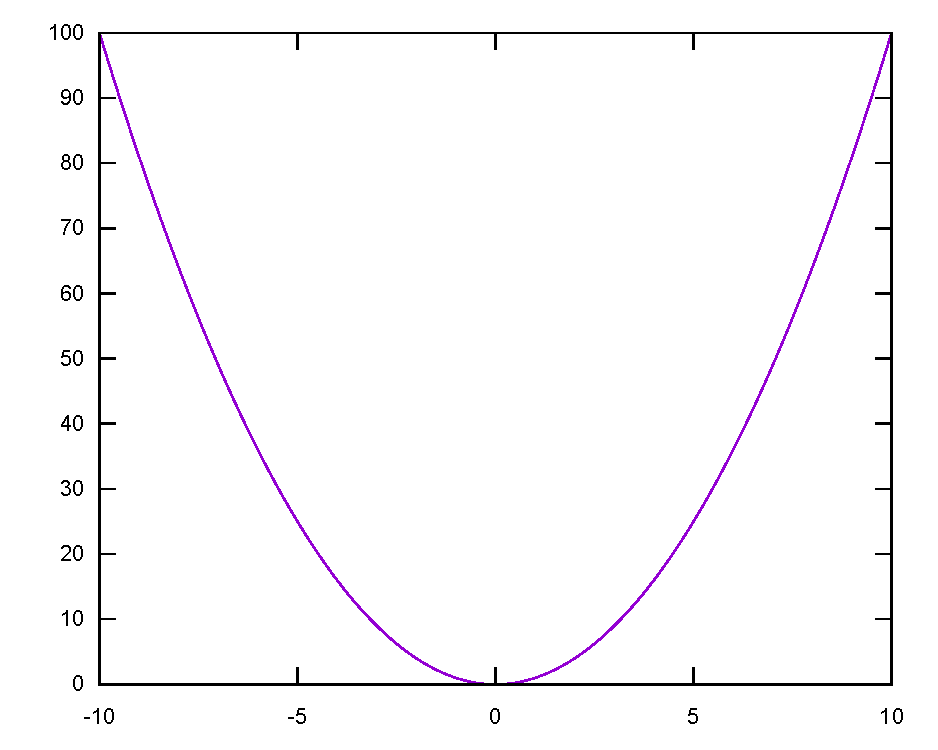
\includegraphics[width=0.65\textwidth]{plots/square.pdf}
        \end{figure}
\end{minipage}
\begin{minipage}{\textwidth}
  \item[mexican\_hat] 4th degree polynomial that looks like a mexican hat, with 2 minima.
        \[
        (x-4)^{2}(x + 4)^{2}
        \]
        \begin{figure}[H]
          \centering
          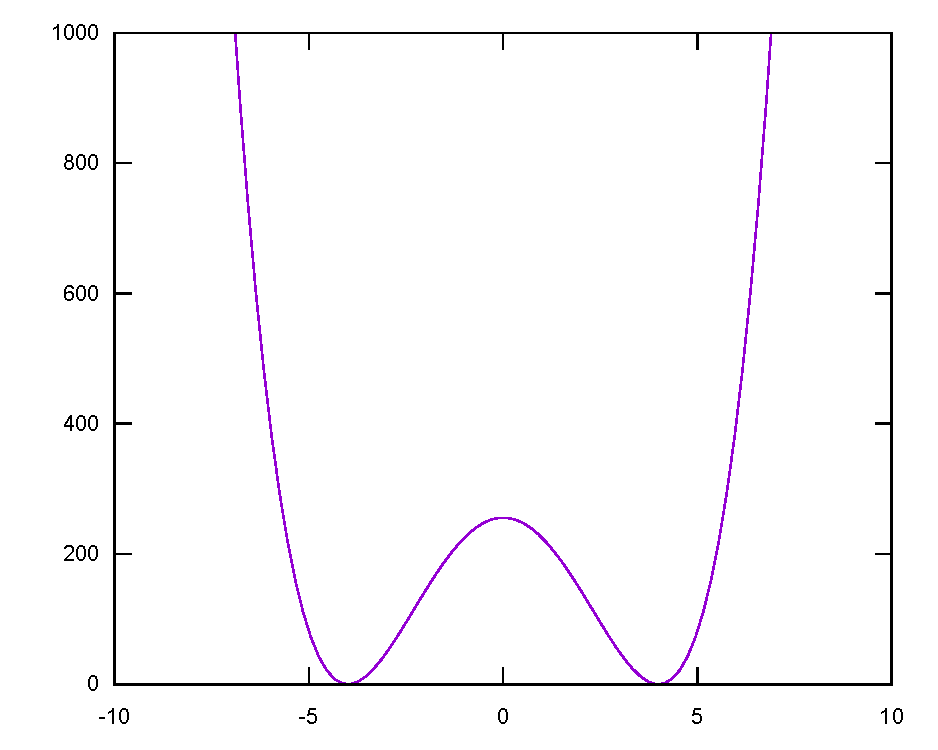
\includegraphics[width=0.65\textwidth]{plots/mexican_hat.pdf}
        \end{figure}
\end{minipage}
\begin{minipage}{\textwidth}
  \item[double\_mexican\_hat] 6th degree polynomial that has 3 minima.
        \[
        (x-4)^{2}x^{2}(x + 4)^{2}
        \]
        \begin{figure}[H]
          \centering
          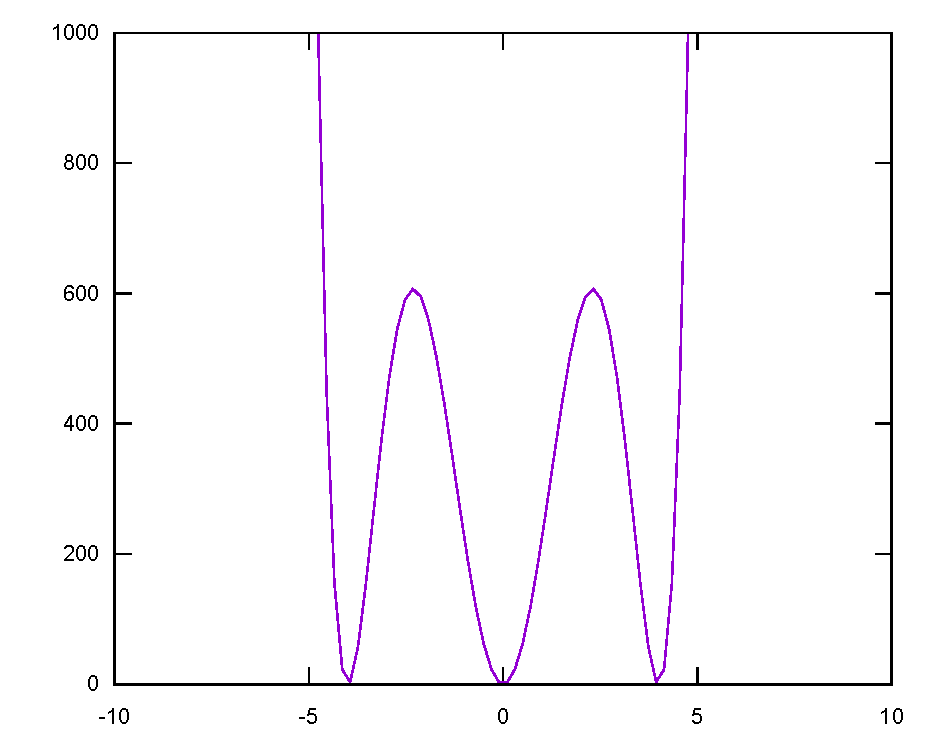
\includegraphics[width=0.65\textwidth]{plots/double_mexican_hat.pdf}
        \end{figure}
\end{minipage}
\begin{minipage}{\textwidth}
  \item[triple\_mexican\_hat] 8th degree polynomial that has 4 minima.
        \[
        (x - 6)^{2}(x - 3)^{2}(x + 3)^{2}(x + 6)^{2}
        \]
        \begin{figure}[H]
          \centering
          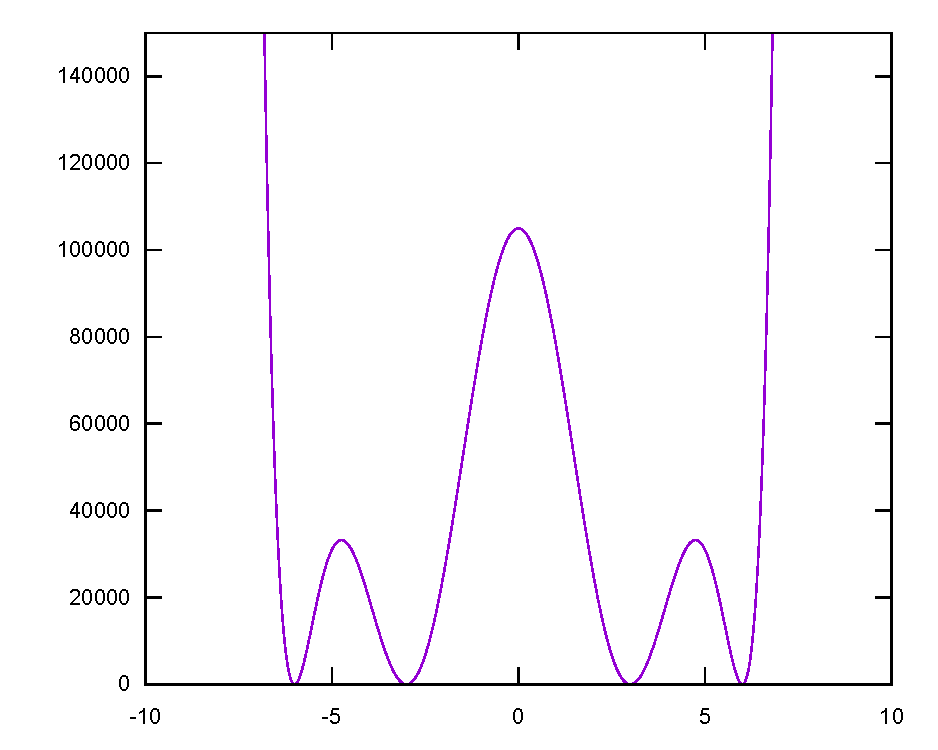
\includegraphics[width=0.65\textwidth]{plots/triple_mexican_hat.pdf}
        \end{figure}
\end{minipage}
  \item[smooth\_step] Step function that goes to \rustinline{ENERGY_INF} outside the interval $(-5, 5)$. Joints were added at $\pm 5$ to make the function differentiable.
\end{description}

\subsection{Custom Potentials}\label{sec:custom-potentials}
To create a custom potential you'll have to define a function like shown below.
\begin{rustcode}
fn my_potential(x: f64) -> f64 {
    return /*some calculation*/;
}
\end{rustcode}
\rustinline{my_potential} is the name that you can choose and have to use later when you're passing it to \rustinline{WaveFunction::new}.
\rustinline{/*some calculation*/} can be any Rust code that results in a \rustinline{f64}.
\\
\subsubsection{Examples}
Negative bell curve ($-e^{-x^{2}} + 1$)
\begin{rustcode}
fn neg_bell(x: f64) -> f64 {
    return -(-x.powi(2)).exp();
}
\end{rustcode}

\noindent General polynomial (might not work for all configurations)
\begin{rustcode}
const COEFFICIENTS: [f64;4] = [a, b, c, d]
fn polynom(x: f64) -> f64 {
    let mut result = 0.0;
    for n in 0..COEFFICIENTS.len() {
        result += x.powi(n) * COEFFICIENTS[n];
    }
    return result;
}
\end{rustcode}
You need to set values for \rustinline{a}, \rustinline{b}, etc. and they need to be floating point numbers or you'll get error E0308. For example \rustinline{1} would cause an error but \rustinline{1.0}
or \rustinline{3.141} are correct. You can add even more coefficients if you'd like. The 4 in the square brackets is the degree of the polynomial plus 1.
The potential above would mathematically be $a + b x + c x^{2} + d x^{3}$.


\begin{appendix} %Anhang falls nötig
%
\chapter{Detailed Calculations}
\section{Proofs}
\subsection{Smoothness of Transitionfunction}\label{proof:joint}
Given that
\begin{align}
  f: \mathbb{R} \rightarrow \mathbb{C} \\
  g: \mathbb{R} \rightarrow \mathbb{C} \\
  \{f, g\} \in C^{1} \\
  \{\alpha, \delta\} \in \mathbb{C}
\end{align}
define \hspace*{\fill}~\citep{hall2013quantum}
\begin{align}
  \chi(x) = \sin^{2}\left(\cfrac{\pi(x - \alpha)}{2\delta}\right) \\
  (f \sqcup g)(x) = f(x) + (g(x) - f(x)) \chi(x)
\end{align}
and proof that
\begin{align}
  \label{eq:deriv-f}
  \cfrac{d(f \sqcup g)}{dx}(\alpha) = \cfrac{df}{dx}(\alpha) \\
  \label{eq:deriv-g}
  \cfrac{d(f \sqcup g)}{dx}(\alpha + \delta) = \cfrac{dg}{dx}(\alpha + \delta).
\end{align}
Calculate derivatives
\begin{align}
  \deriv{\chi}{x}(x) = \cfrac{\pi}{2 \delta} \sin\left(\cfrac{\pi (x - \alpha)}{\delta}\right)\\
  \deriv{(f \sqcup g)}{x}(x) = \deriv{f}{x}(x) + \left(\deriv{g}{x}(x) - \deriv{f}{x}(x)\right)\chi(x) + (g(x) - f(x))\deriv{\chi}{x}(x).
\end{align}
Note that
\begin{align}
  \deriv{\chi}{x}(\alpha) = 0 \\
  \chi(\alpha) = 0 \\
  \deriv{\chi}{x}(\alpha + \delta) = 0 \\
  \chi(\alpha + \delta) = 1
\end{align}
therefor
\begin{align}
  \deriv{(f \sqcup g)}{x}(\alpha) = \deriv{f}{x}(\alpha) + 0 \left(\deriv{g}{x}(\alpha) - \deriv{f}{x}(\alpha)\right) + 0 (g(x) - f(x)) = \deriv{f}{x}(\alpha)
\end{align}
and
\begin{align}
  \deriv{(f \sqcup g)}{x}(\alpha + \delta) = \deriv{f}{x}(\alpha + \delta) + 1 \left(\deriv{g}{x}(\alpha + \delta) - \deriv{f}{x}(\alpha + \delta)\right) + 0 (g(x) - f(x)) \\
  \deriv{(f \sqcup g)}{x}(\alpha + \delta) = \deriv{f}{x}(\alpha + \delta) + \deriv{g}{x}(\alpha + \delta) - \deriv{f}{x}(\alpha + \delta) = \deriv{g}{x}(\alpha + \delta)~\blacksquare.
\end{align}

\chapter{Data Files}
\section{Energies}
\begin{paracol}{2}

\bashinline{energy.txt}\label{dat:energy-rs}
\begin{lstlisting}
0 1.4143970999546869
1 4.2427225425397275
2 7.071360490007656
3 9.89984218503414
4 12.727855127619105
5 15.55633682264559
6 18.384818517672073
7 21.213143965139928
8 24.041938165049302
9 26.870419860075785
10 29.69843279777794
11 32.52722700257012
12 35.35570869759661
13 38.18372163529877
14 41.012203335208056
15 43.84099753511743
16 46.66901047281958
17 49.49733591540462
18 52.32628637263825
19 55.15445556278185
20 57.98309351024977
21 60.811106452834736
22 63.64005690518555
23 66.46853860021204
24 69.29639528547274
25 72.1247207329406
26 74.95335868040853
27 77.78168412299357
28 80.61047832778574
29 83.43927252769512
30 86.26697296051438
31 89.09561090798232
32 91.92378010300872
33 94.75288680780098
34 97.58121225038602
35 100.40938144541242
36 103.23739438311458
37 106.06587607814106
38 108.89435777316754
39 111.72299572551829
40 114.55178992542766
41 117.38027162045414
42 120.2082845630391
43 123.0364537531827
44 125.86493544820918
45 128.69341714323565
46 131.52174259070352
47 134.35053679061292
48 137.17854972831506
49 140.0071876806658
50 142.83566937569228
\end{lstlisting}
\switchcolumn{}
\bashinline{energies_exact.dat}\label{dat:energy-wsl}
\begin{lstlisting}
0 1.4142135623730951
1 4.242640687119286
2 7.0710678118654755
3 9.899494936611665
4 12.727922061357857
5 15.556349186104047
6 18.38477631085024
7 21.213203435596427
8 24.041630560342618
9 26.870057685088806
10 29.698484809834998
11 32.526911934581186
12 35.35533905932738
13 38.18376618407357
14 41.01219330881976
15 43.84062043356595
16 46.66904755831214
17 49.49747468305833
18 52.32590180780452
19 55.15432893255071
20 57.9827560572969
21 60.81118318204309
22 63.63961030678928
23 66.46803743153548
24 69.29646455628166
25 72.12489168102785
26 74.95331880577405
27 77.78174593052023
28 80.61017305526643
29 83.43860018001261
30 86.2670273047588
31 89.095454429505
32 91.92388155425118
33 94.75230867899738
34 97.58073580374356
35 100.40916292848975
36 103.23759005323595
37 106.06601717798213
38 108.89444430272833
39 111.72287142747452
40 114.5512985522207
41 117.3797256769669
42 120.20815280171308
43 123.03657992645928
44 125.86500705120547
45 128.69343417595167
46 131.52186130069785
47 134.35028842544403
48 137.17871555019022
49 140.00714267493643
50 142.83556979968262
\end{lstlisting}
\end{paracol}

\chapter{Source Code}
\begin{figure}[H]
  \label{fig:uml-arch}
  \centering
  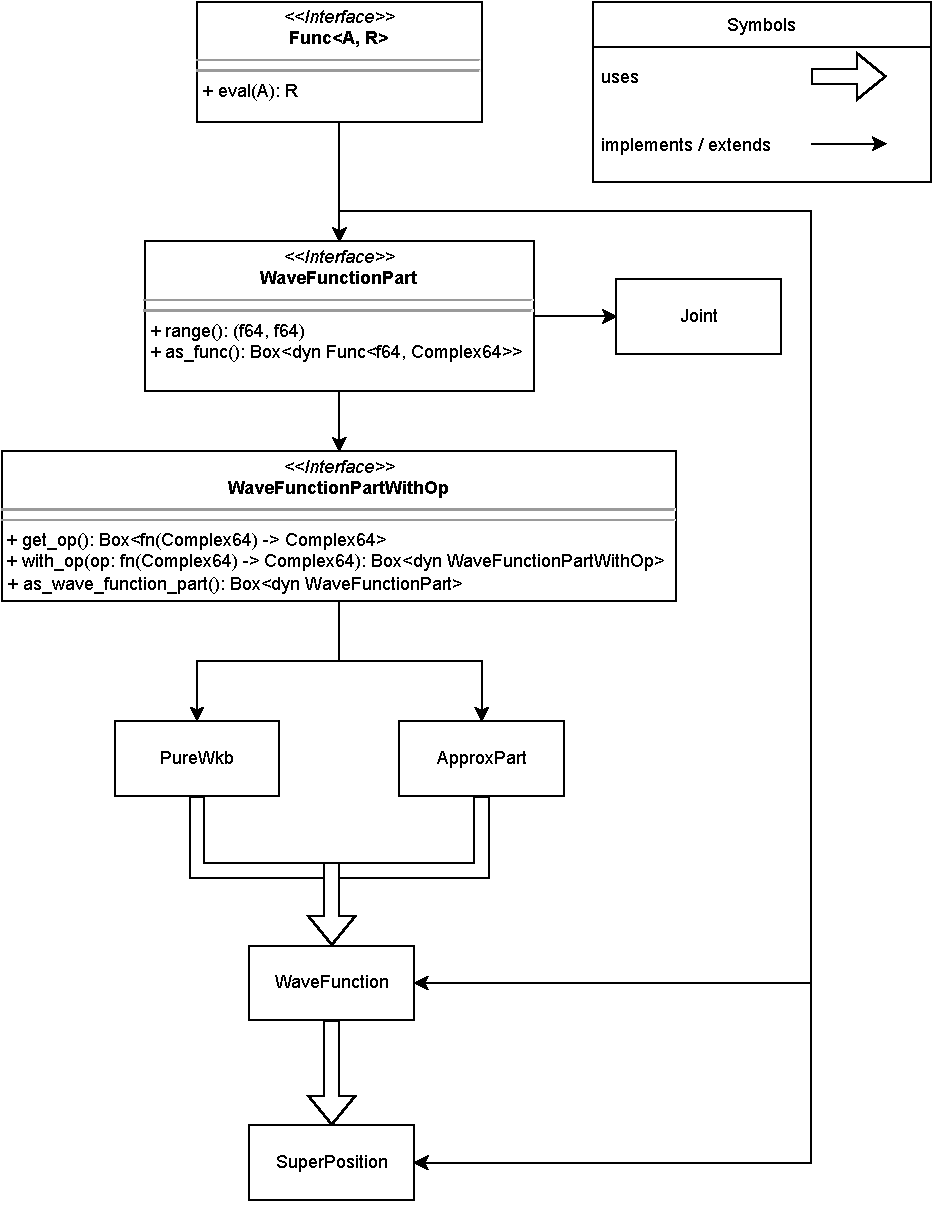
\includegraphics[width=\textwidth]{program_architecture.pdf}
  \caption{UML diagram of program architecture}
\end{figure}

The source code is also available on the authors GitHub \\
\url{https://github.com/Gian-Laager/Schroedinger-Approximation}\\[3ex]

{\noindent \large \bfseries src/main.rs}
\lstinputlisting[language=Rust]{code/src/main.rs}

\vspace*{3ex}
{\noindent \large \bfseries src/airy.rs}
\lstinputlisting[language=Rust]{code/src/airy.rs}

\vspace*{3ex}
{\noindent \large \bfseries src/airy\_wave\_func.rs}
\lstinputlisting[language=Rust]{code/src/airy_wave_func.rs}

\vspace*{3ex}
{\noindent \large \bfseries src/check.rs}
\lstinputlisting[language=Rust]{code/src/check.rs}

\vspace*{3ex}
{\noindent \large \bfseries src/energy.rs}
\lstinputlisting[language=Rust]{code/src/energy.rs}

\vspace*{3ex}
{\noindent \large \bfseries src/integrals.rs}
\lstinputlisting[language=Rust]{code/src/integrals.rs}

\vspace*{3ex}
{\noindent \large \bfseries src/main.rs}
\lstinputlisting[language=Rust]{code/src/main.rs}

\vspace*{3ex}
{\noindent \large \bfseries src/newtons\_method.rs}
\lstinputlisting[language=Rust]{code/src/newtons_method.rs}

\vspace*{3ex}
{\noindent \large \bfseries src/plot.rs}
\lstinputlisting[language=Rust]{code/src/plot.rs}

\vspace*{3ex}
{\noindent \large \bfseries src/potentials.rs}
\lstinputlisting[language=Rust]{code/src/potentials.rs}

\vspace*{3ex}
{\noindent \large \bfseries src/tui.rs}
\lstinputlisting[language=Rust]{code/src/tui.rs}

\vspace*{3ex}
{\noindent \large \bfseries src/turning\_points.rs}
\lstinputlisting[language=Rust]{code/src/turning_points.rs}

\vspace*{3ex}
{\noindent \large \bfseries src/utils.rs}
\lstinputlisting[language=Rust]{code/src/utils.rs}

\vspace*{3ex}
{\noindent \large \bfseries src/wave\_function\_builder.rs}
\lstinputlisting[language=Rust]{code/src/wave_function_builder.rs}

\vspace*{3ex}
{\noindent \large \bfseries src/wkb\_wave\_func.rs}
\lstinputlisting[language=Rust]{code/src/wkb_wave_func.rs}

\vspace*{3ex}
{\noindent \large \bfseries lib/build.sh}
\lstinputlisting[language=bash]{code/lib/build.sh}

\vspace*{3ex}
{\noindent \large \bfseries lib/go.mod}
\lstinputlisting[]{code/lib/go.mod}

\vspace*{3ex}
{\noindent \large \bfseries lib/main.go}
\lstinputlisting[language=Go]{code/lib/main.go}

\vspace*{3ex}
{\noindent \large \bfseries build.rs}
\lstinputlisting[language=Rust]{code/build.rs}

\vspace*{3ex}
{\noindent \large \bfseries Cargo.toml}
\lstinputlisting[language=Rust]{code/Cargo.toml}

\vspace*{3ex}
{\noindent \large \bfseries energy.wsl}
\lstinputlisting[]{code/energy.wsl}

\vspace*{3ex}
{\noindent \large \bfseries exact.wsl}
\lstinputlisting[]{code/exact.wsl}

\end{appendix}
\chapter*{Bildquellen}
%
Wo nicht anders angegeben, sind die Bilder aus dieser Arbeit selbst erstellt worden.
%
\bibliographystyle{plainnatromer}
\bibliography{marbeit}

%
\chapter*{Selbständigkeitserklärung}
%
Hiermit bestätige ich, Gian Laager, meine Maturaarbeit selbständig verfasst und alle Quellen angegeben zu haben.\\\newline
Ich nehme zur Kenntnis, dass meine Arbeit zur Überprüfung der korrekten und vollständigen Angabe der Quellen mit Hilfe einer Software (Plagiaterkennungstool) geprüft wird. Zu meinem eigenen Schutz wird die Software auch dazu verwendet, später eingereichte Arbeiten mit meiner Arbeit elektronisch zu vergleichen und damit Abschriften und eine Verletzung meines Urheberrechts zu verhindern. Falls Verdacht besteht, dass mein Urheberrecht verletzt wurde, erkläre ich mich damit einverstanden, dass die Schulleitung meine Arbeit zu Prüfzwecken herausgibt.\\\newline
Ort\hspace{4cm} Datum\hspace{4cm}  Unterschrift
%
\end{document}
